\documentclass[a4paper,12pt]{report}

\usepackage[utf8]{inputenc}
\usepackage[T1]{fontenc}
\usepackage{array}
\usepackage{amsmath}
\usepackage[english]{babel}
\usepackage{bm}
\usepackage{graphicx}
\usepackage[a4paper]{geometry}
\usepackage[colorlinks=true,urlcolor=blue,linkcolor=blue]{hyperref}
\usepackage{url}
\usepackage[nottoc,numbib]{tocbibind}
\usepackage{color}
\usepackage{epstopdf}
\usepackage{xcolor}
\usepackage{rotating}
%\usepackage{wrapfig,booktabs}
\usepackage[backend=biber,style=phys]{biblatex}
\usepackage{upgreek}

\addbibresource{../Bibliography.bib}

\makeatletter
	\renewcommand{\thechapter}{\Roman{chapter}}
\makeatother

\begin{document}

\chapter{Magneto-optical study of Cr-doped CdTe quantum dots\label{MagOptStud}}

	In this chapter, we will study the photoluminescence of a II-VI quantum dot containing a single Chromium atom. We saw in the Sec.~\ref{CrSemiCon} that the magnetic anisotropy of the spin leads to a zero magnetic field splitting of the $0$, $\pm 1$ and $\pm 2$ states. In a neutral Cr-doped quantum dot, such an anisotropy is induced by the bi-axial strains in the plane of the dots. Probing optically the dot, it results that exchange interaction is enough to see the effect of the presence of a single Cr spin in the QD. Studying the magnetic-field dependence of the quantum dots photoluminescence also shows the influence of the symmetry on carrier-Cr spin coupling.
	
	The chapter is organized as follows. First, we present the photoluminescence of several dots, extracting the Cr energy structure from it. Several features of this luminescence is then discussed. The study of the dot emission under magnetic field confirm the chosen energy structure. In the second section, we explain the model in more details, extracting parameters from the magneto-optics experiment, and examining its prediction for a different type of QD. Finally, we present and give a possible explanation to dots not explained by the model presented in this chapter.

	\section{Strained quantum dots containing an individual Cr atom}
	
		\subsection{Energy structure of a Cr in a quantum dot}
		
		Using the procedure described in the Sec.~\ref{SKGrowth}, we randomly incorporated Cr atoms in CdTe/ZnTe quantum dots, adjusting the density of the Cr atoms to be roughly equal to the density of dots, in order to get QDs containing 0, 1 or a few Cr atoms. The photoluminescence (PL) of individual QDs, induced by optical excitation with a dye laser tuned on resonance with an excited state of the dots, is studied by optical micro-spectroscopy.
		
	\begin{figure}[h!]
	\begin{center}
		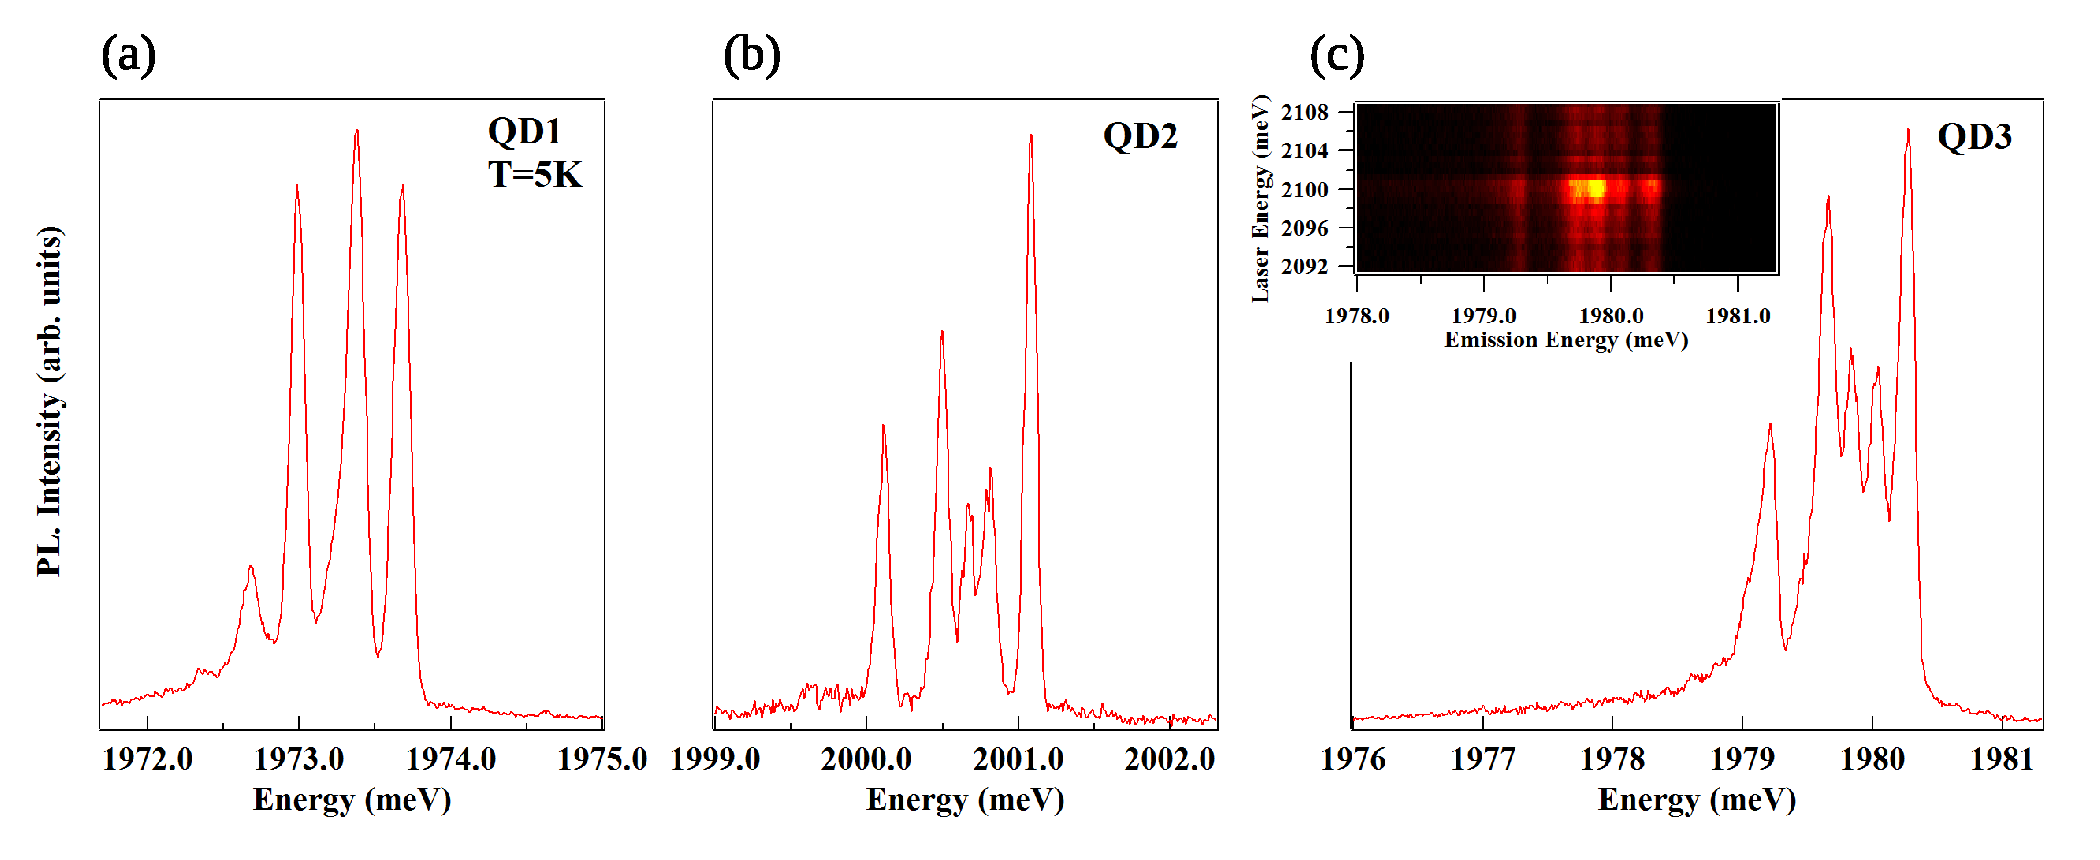
\includegraphics[width=15cm]{Pictures/Spectras.eps}
	\end{center}
	\caption{PL of (a) QD1, (b) QD2 and (c) QD3 X-Cr complex at low temperature (T=5K). Inset presents the PLE map of this QD, showing a sharp quasi-resonant state for an excitation at 2100 meV.}
	\label{SpectraX}
	\end{figure}

	Low temperature (T=5K) PL of the neutral exciton (X-Cr) of several QD doped with a single Cr are reported in Fig.~\ref{SpectraX}. Four emission lines are observed as shown in QD1, with the central peak being split in some QDs, such as QD2 and QD3. Scanning with an energy tunable laser, we saw that all the peaks share a common quasi-resonant state, where all are at a maximum intensity, as highlighted in the inset of Fig.~\ref{SpectraX}(c). This is an indication that they originate from the same dot. Variations in the relative intensities of the peaks are observed in different dots. The lowest energy peak is shown as getting more intense  when the splitting of the central peak get wider.

	\begin{figure}[h!]
	\begin{center}
		\includegraphics[width=10cm]{Pictures/EnLvlantiferro.png}
	\end{center}
	\caption{Illustration of the energy levels of the ground state (Cr), the bright exciton states ($|\pm1\rangle$) coupled to the spin of a Cr (X-Cr) and dominant PL transitions ($\sigma$+, $\sigma$-). The states $S_z = |\pm2\rangle$ cannot be populated through thermalization, and thus the recombination channel are not shown on this schema.}
	\label{CrEnergyStruct}
	\end{figure}

	In a II-VI semiconductor, the orbital momentum of the Cr connects the spin of the atom to its local strain environment through the modification of the crystal field and the spin-orbit coupling. For biaxial strain in the (001) plane, the ground state of a Cr spin is split by a strain induced magnetic anisotropy term ${\cal H}_{Cr,\varepsilon_\parallel}=D_0S^2_z$ (see Sec.~\ref{CrSemiCon}). It was deduced from electron paramagnetic resonance of bulk Cr-doped CdTe that $D_0$ is positive for compressive biaxial strain~\cite{EPRCr}. In a self-assembled CdTe/ZnTe QD with large in-plane strain, the Cr spin energy levels are split from $S_z=|0\rangle$ at low energy (Fig.~\ref{CrEnergyStruct}). A value of $D_0$ in the 1 meV range can be expected for a CdTe layer strained on a ZnTe substrate, as shown in Sec.~\ref{CrSemiCon}.
	
	When an electron-hole (e-h) pair is injected in a Cr-doped QD, the bright excitons are split by the exchange interaction between the spins of Cr and carriers. In flat self-assembled QDs, the heavy-holes and light-holes are separated in energy by the biaxial strain and the confinement. In a first approximation, the ground state in such QD is a pure heavy-hole ($J_z$=$\pm$3/2) exciton and the exchange interaction with the Cr spin S is described by the spin Hamiltonian 
	\begin{align}
		{\cal H}_{c-Cr}=I_{eCr}\vec{S}\cdot\vec{\sigma}+I_{hCr}S_zJ_z
	\end{align}		
with $\bm{\upsigma}$ the electron spin and $J_z$ the hole spin operator. $I_{eCr}$ and $I_{hCr}$ are, respectively, the exchange integrals of the electron and the hole spins with the Cr spin. These exchange energies depend on the exchange constant of the Cr $3d$ electrons of with the CdTe carriers and on the overlap of the Cr atom with the confined carriers. Even though the exchange interaction of the Cr spin with both electron and hole is ferromagnetic in most II-VI semiconductor~\cite{MacCdCrSD0beta,KacmanD0alphabetaIIVI,MacspdexchCr}, the hole-Cr interaction is supposed to be anti-ferromagnetic here. This will be further discussed in Sec.~\ref{MagOptCr}. A typical exchange constant 4 to 5 times larger for the holes than for the electrons is also expected in CdTe~\cite{DMSCrExchInt,CdCrSExchInt}.

	\begin{figure}[h!]
	\begin{center}
		\includegraphics[width=15cm]{Pictures/LinPol.png}
	\end{center}
	\caption{(a) Low temperature PL of QD2 recorded along two orthogonal directions. (b) Linear polarization PL intensity map of QD2. The 0$^{\circ}$ polarization angle corresponds to an emission polarized along the QD cleavage axis, either $110$ or $1\bar{1}0$. (c) Illustration of the energy levels of the ground state (Cr), the bright exciton states ($|\pm1\rangle$) coupled to the spin of a Cr (X-Cr), showing the splitting of the central peak via the bright exciton coupling, and dominant PL transitions ($\sigma$+ (blue), $\sigma$- (red) and $\pi$ (green and black)).}
	\label{CrLinPolar}
	\end{figure}
	
	For highly strained CdTe/ZnTe QDs with a weak hole confinement, the strain induced energy splitting of the Cr spin $D_0S^2_z$ is much larger than the exchange energy with the confined carriers ($D_0\gg |I_{hCr}|>|I_{eCr}|$). The exchange interaction with the exciton acts as an effective magnetic field which further splits the Cr spins states S$_z$=$\pm$1 and S$_z$=$\pm$2. The resulting X-Cr energy levels are presented in Fig.~\ref{CrEnergyStruct}. The exciton recombination does not affect the Cr atom and its spin is conserved during the optical transitions. Consequently, the large strain induced splitting of the Cr spin is not directly observed in the optical spectra. However, at low temperature, the Cr spin thermalize on the low energy states $S_z$=0 and $S_z$=$\pm$1. This leads to a PL dominated by three contributions: a central line corresponding to $S_z$=0 and the two outer lines associated with S$_z$=$\pm$1 split by the exchange interaction with the carriers.
	
	Cr-doped quantum dots exhibit a linear polarization dependence, as presented in Fig.~\ref{CrLinPolar}. The central line ($S_z$=0) is split and linearly polarized along two orthogonal directions. As in non-magnetic QDs, this results from a coupling of the two bright excitons $|\pm1\rangle$ by (i) the short range e-h exchange interaction in the presence of valence band mixing and/or (ii) the long-range e-h exchange interaction in a QD with an in-plane shape anisotropy~\cite{SplitInvTh}. This anisotropic e-h exchange energy mixes the bright exciton associated with the same Cr spin state, inducing an extra splitting between them. The mixing is maximum for the central pair of bright excitons (S$_z$=0) which are initially degenerated. The outer lines are also slightly linearly polarized but the influence of the e-h exchange interaction is attenuated by the initial splitting of the $|\pm1\rangle$ excitons induced by the exchange interaction with the Cr spin$S_z$=$\pm1$.	

	\begin{figure}[h!]
	\begin{center}
		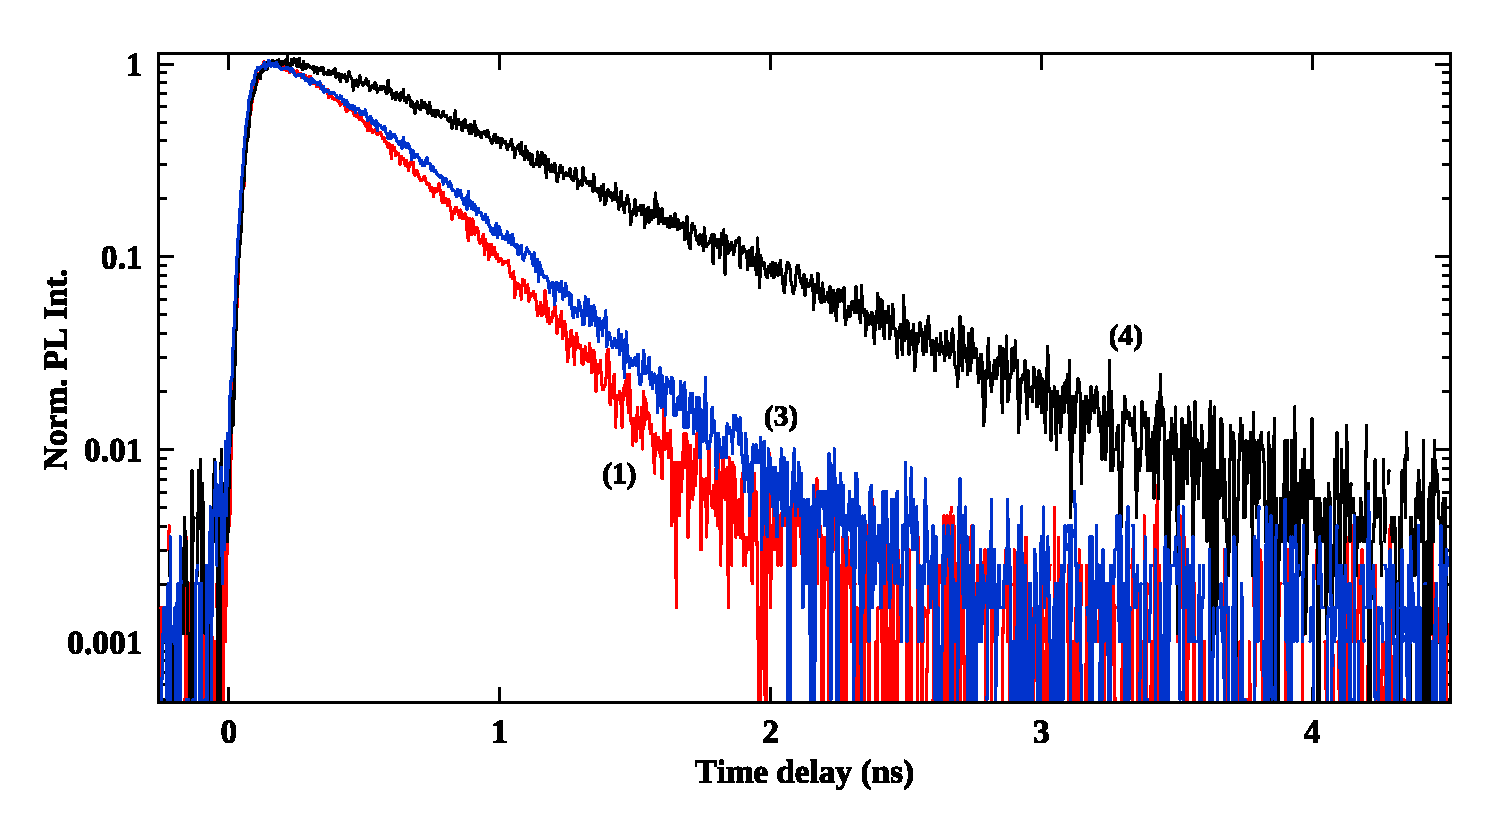
\includegraphics[width=10cm]{Pictures/Decay.eps}
	\end{center}
	\caption{Time resolved PL of QD2 taken on two exterior peaks, attributed to $|S_z = +1\rangle$ and $|S_z = -1\rangle$ (noted (1) and (3) in Fig.~\ref{CrLinPolar}(a)), and the lower energy one (noted (4)).}
	\label{CrDecay}
	\end{figure}

	In order to identify the lower energy peak ((4) in Fig.~\ref{CrLinPolar}(a)), we took the time resolved photoluminescence of the emission peaks, presented in Fig.~\ref{CrDecay}. One can notice that the line (4) present a decay time about twice as long as the high energy peak. A long recombination time is one of the characteristics of a dark exciton emission~\cite{DELongLifetime}. Under normal circumstances, the recombination of such a state is non-radiative. However, it is possible to observe a dark exciton recombination emitting a photon in low symmetry quantum dot~\cite{DELum}. This hypothesis will be confirmed by the magneto-optical study of the dot presented in Fig.~\ref{CrMagOptExp} and \ref{CrMagOptMod}.
	
	\begin{figure}[h!]
	\begin{center}
		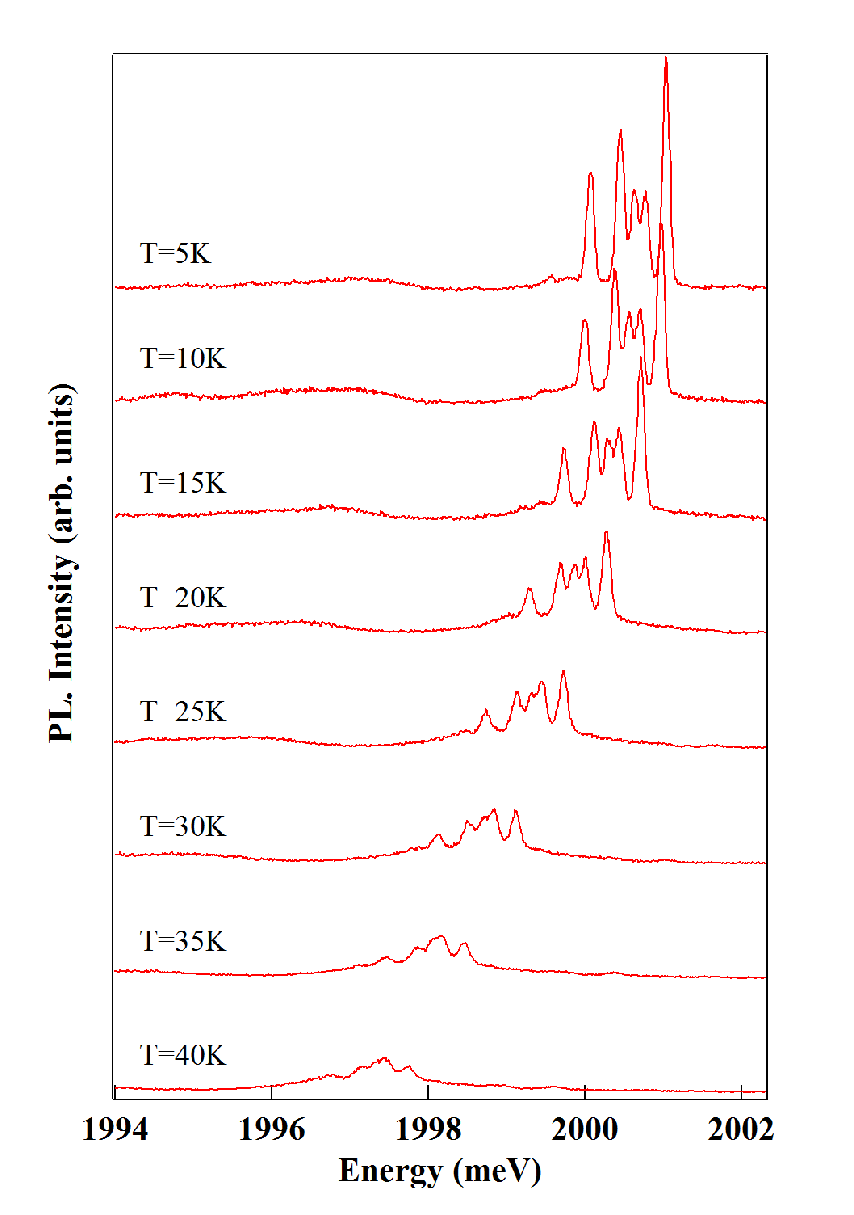
\includegraphics[width=15cm]{Pictures/Temp.eps}
	\end{center}
	\caption{Temperature evolution from T=5K to T=40K of (a) QD2 PL and (b) the PL of a QD with a good thermalisation on the low energy states (QD4). Even at 40K, $|S_z = \pm2\rangle$ states do not appear.}
	\label{CrTemp}
	\end{figure}	
	
	Since the absence of PL on $|\pm2\rangle$ is linked to their impossibility to be thermally populated, one could expect to see their emission at higher temperature. Fig.~\ref{CrTemp} presents the emission of two dots in function of the temperature. With the increase of the temperature, we observe a significant line broadening induced by the interaction with acoustic phonons. In order to keep a significant PL intensity and resolved PL lines, we limited our investigation to temperature below 50K. The figure of the emission change dramatically with the temperature. The intensity of the exterior peaks, associated with the states $S_z = |\pm1\rangle$, fell quickly while the emission of the $S_z = |0\rangle$ stays intense until higher temperature. This is an unexpected picture, since the temperature should allow the higher energy states $|\pm1\rangle$ to be more populated by emptying the ground state, when the opposite is sawn in the experiments. Moreover, even at high temperature, the $S_z = |\pm2\rangle$ states doesn't appears.

%	\begin{sidewaysfigure}
%	\begin{center}
%		\includegraphics[width=20cm]{Pictures/FullPLE}
%	\end{center}
%	\caption{(a) Map of QD2 PL under a scan in laser energy close to the dot emission in $\sigma -$ detection. Several interesting points are highlighted on zoom on each side of this whole map. (b) Map of the first few meV of the scan, showing the phonon replica. The emission integrated intensity in function of the laser energy is plotted in (c) (black curve) along with the PL spectra of QD2 (red curve). (d) - (f) present a zoom in a larger band at higher excitation energy in $\pi$,  $\sigma +$ and $\sigma -$ respectively. (g) Zoom on a particular excited state presented a splitting inversion, presented here in $\pi$ detection.}
%	\label{CrPLE}
%	\end{sidewaysfigure}


		\subsection{Excited states of a Cr-doped QD}
			
	\begin{figure}[h!]
	\begin{center}
		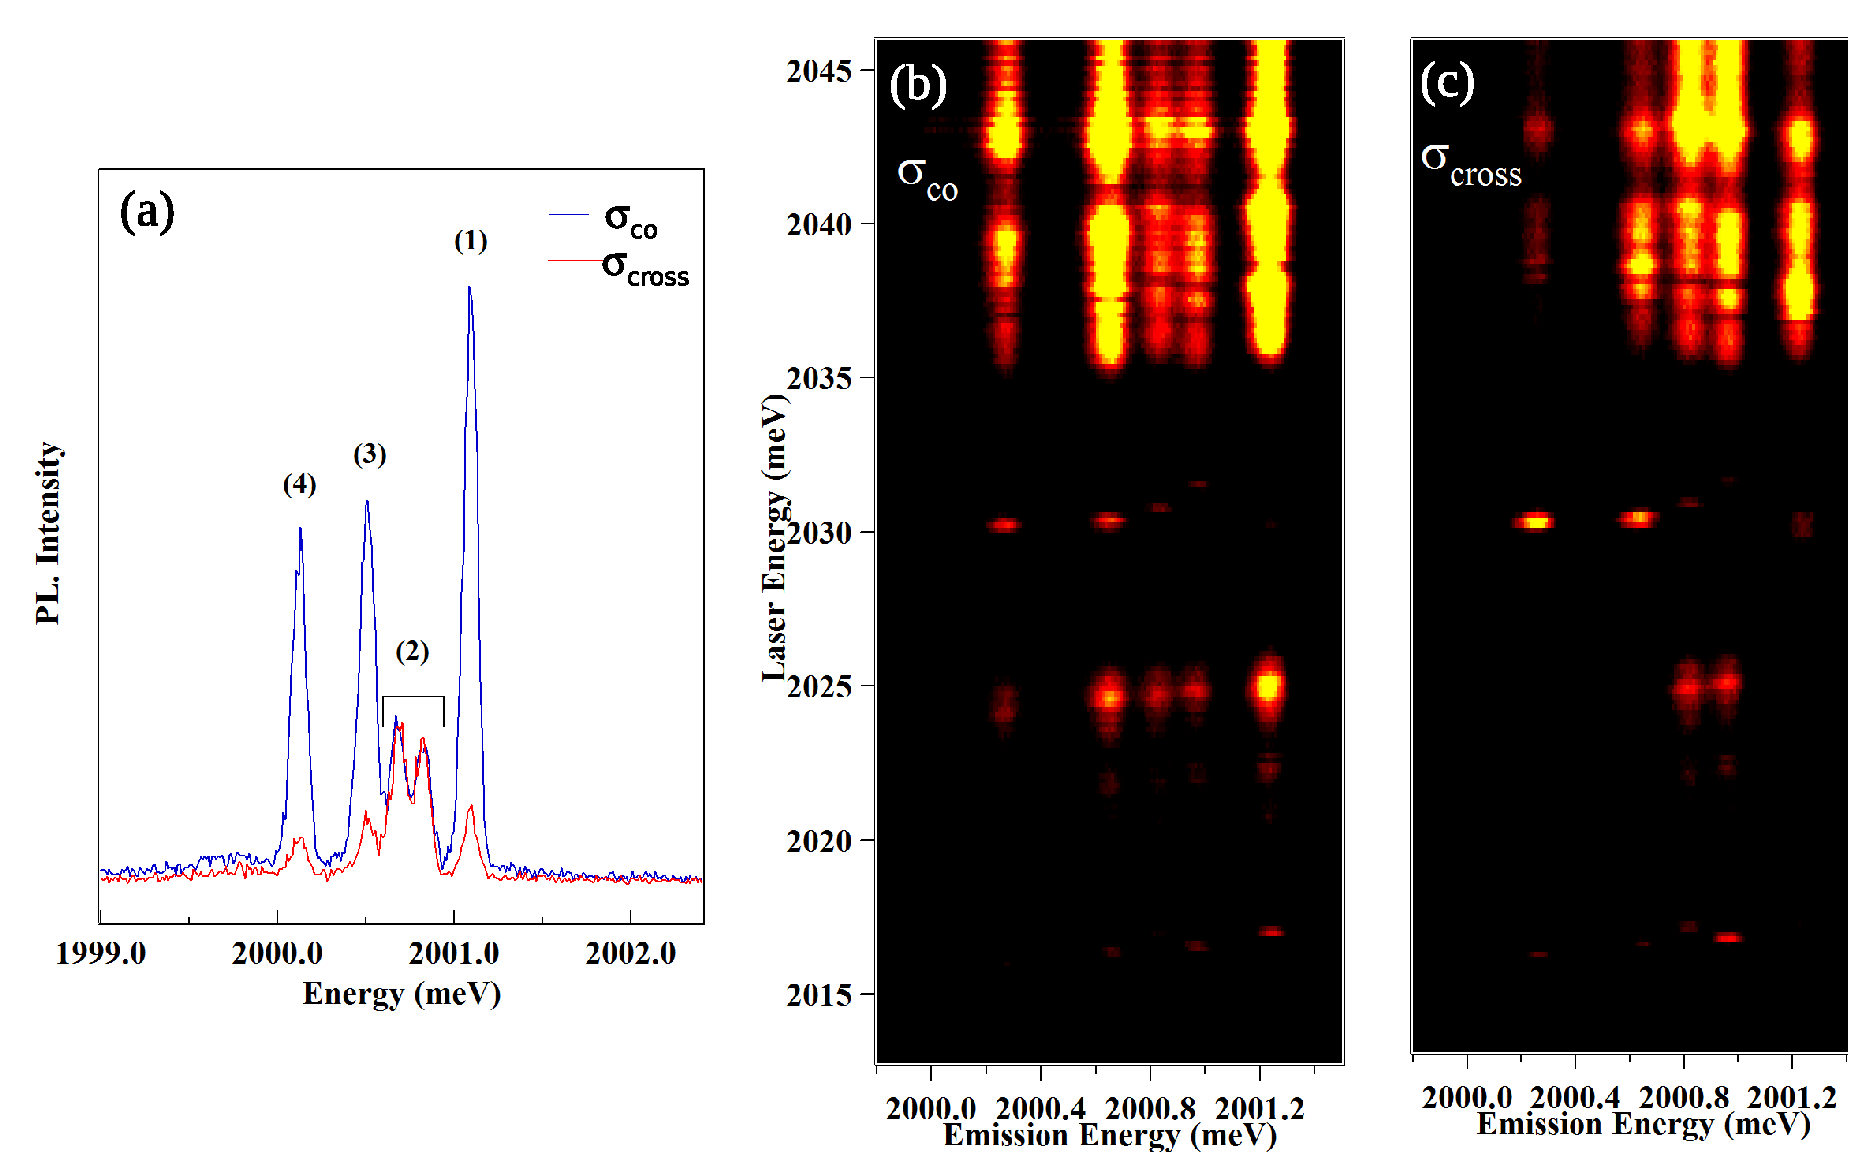
\includegraphics[width=15cm]{Pictures/PLEDotPres.eps}
	\end{center}
	\caption{(a) PL spectra of the exciton in QD2 (X-Cr) for co-circularly (blue) and cross-circularly (red) polarized excitation/detection [À VÉRFIER : taken on the 2175 meV quasi-resonant state]. (b) - (c) PLE map between 2046 meV and 2013 meV presenting several excited states, detecting in $\sigma_{co}$ (b) and $\sigma_{cross}$ (c).}
	\label{PLEDotPres}
	\end{figure}

	In order to study the different excited states presented by a QD doped with a single Cr atom, we took the PLE of QD2 starting close to the energy of the dot's emission. The dot spectra is presented in Fig.~\ref{PLEDotPres}(a) in both $\sigma$ polarizations. The central peaks do not show dependency in circular polarization, which is coherent with their linear polarization dependency presented in Fig.~\ref{CrLinPolar}(a) and (b). The excitation laser is $\sigma$+ polarized in order to control the spin of the injected exciton. The exterior peaks emission being in $\sigma$+ polarization shows that there is no spin flip of the exciton before recombination.
	
	Fig.~\ref{FullPLE}(a) presents the entire PLE of QD2 X-Cr complex. One can note several excited states along the scan.
	
	\begin{figure}[h!]
	\begin{center}
		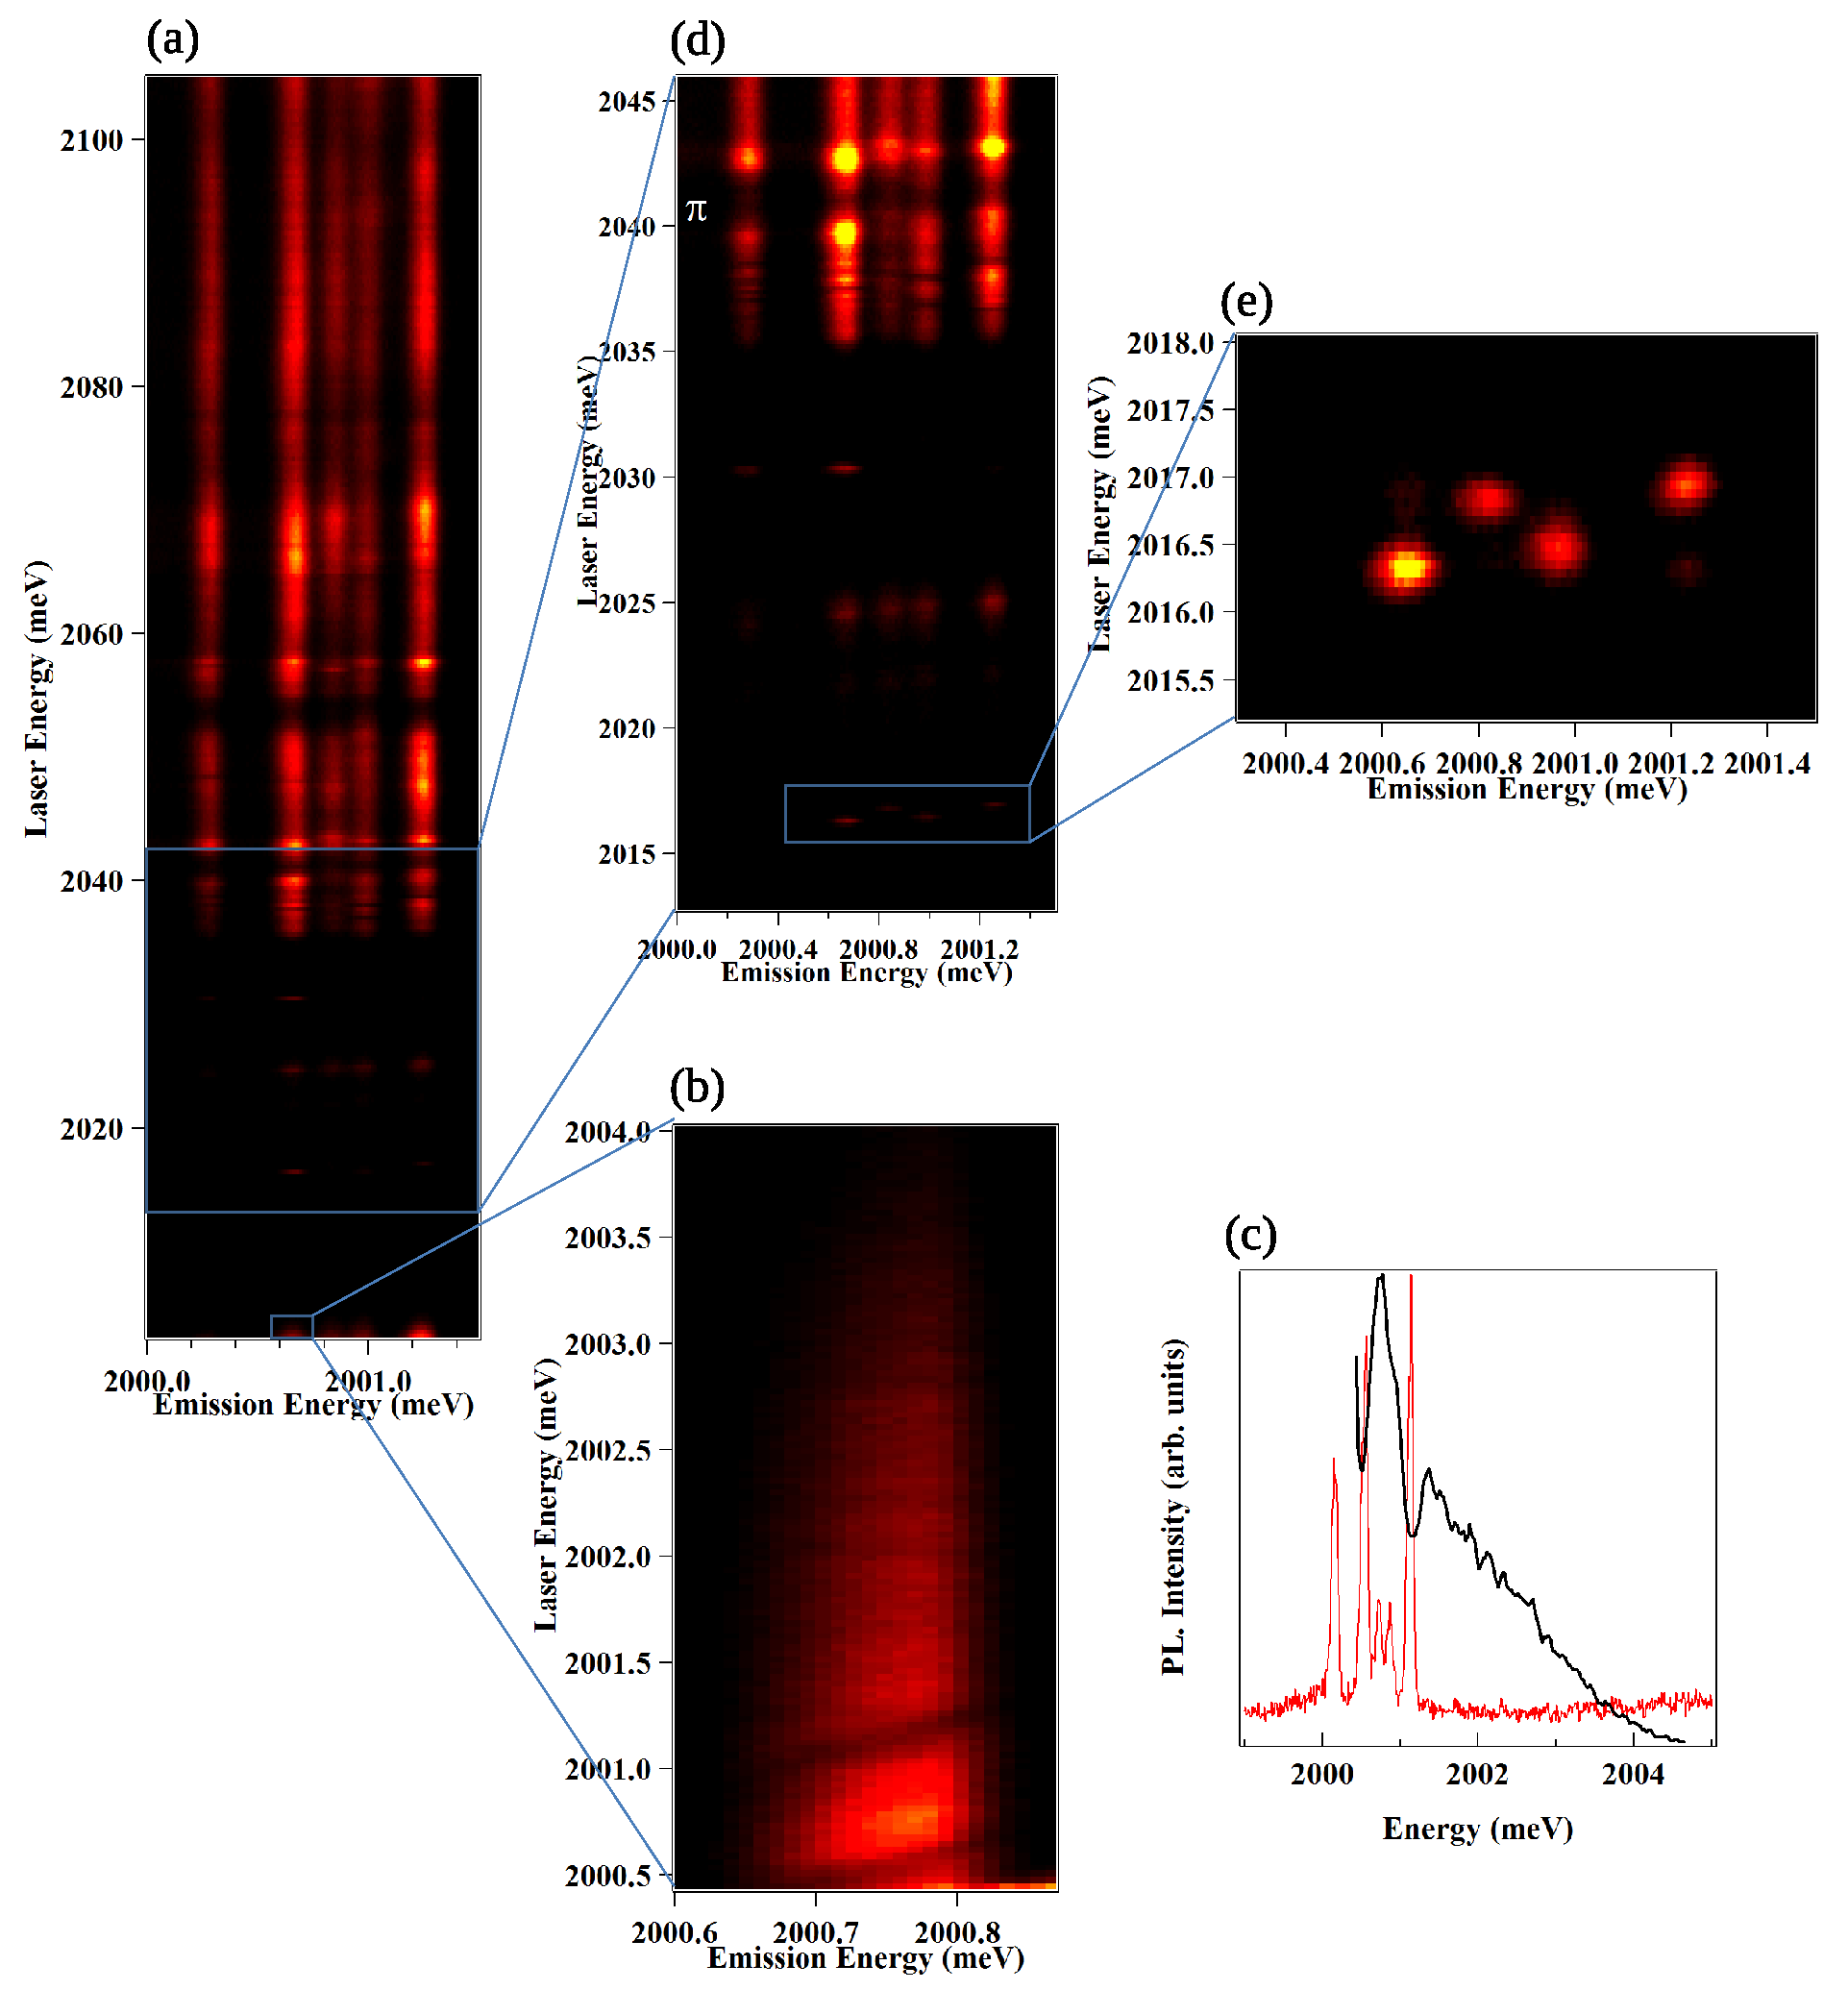
\includegraphics[width=14cm]{Pictures/FullPLEv2.eps}
	\end{center}
	\caption{(a) QD2 X-Cr PLE map in $\sigma_{cross}$ polarization. Several excited states are highlighted. (b) PLE scan of the lower energy peak, taken close to the QD emission energy, showing the phonon replica taken in $\pi$ detection. The emission integrated intensity in function of the laser energy is plotted in (c) (black curve) along with the PL spectra of QD2 taken in $\sigma_{co}$ polarization. (d) PLE map between 2046 meV and 2013 meV presenting several excited, detecting in $\pi$. (d) Zoom in a particular excited state presented a splitting inversion, taken in $\pi$ detection.}
	\label{FullPLE}
	\end{figure}
	
	The first remarkable feature of this scan is the really long luminescence of the acoustic phonon replica. As shown on the zoom in Fig.~\ref{FullPLE}(b), the probed peak continues to emit with an excitation several millielectronvolt above the excited state, remaining visible until 2004 meV. One can also see two sharp intensity diminutions in this emission. Mapping the intensity of the phonon replica to the quantum dot spectrum (Fig.~\ref{FullPLE}(c)), it evidence that these diminutions happens when the laser is in resonance with a QD emission line. The absorption then preferentially occurs in this resonantly excited state than in the acoustic phonon band.
	
%	\begin{figure}[h!]
%	\begin{center}
%		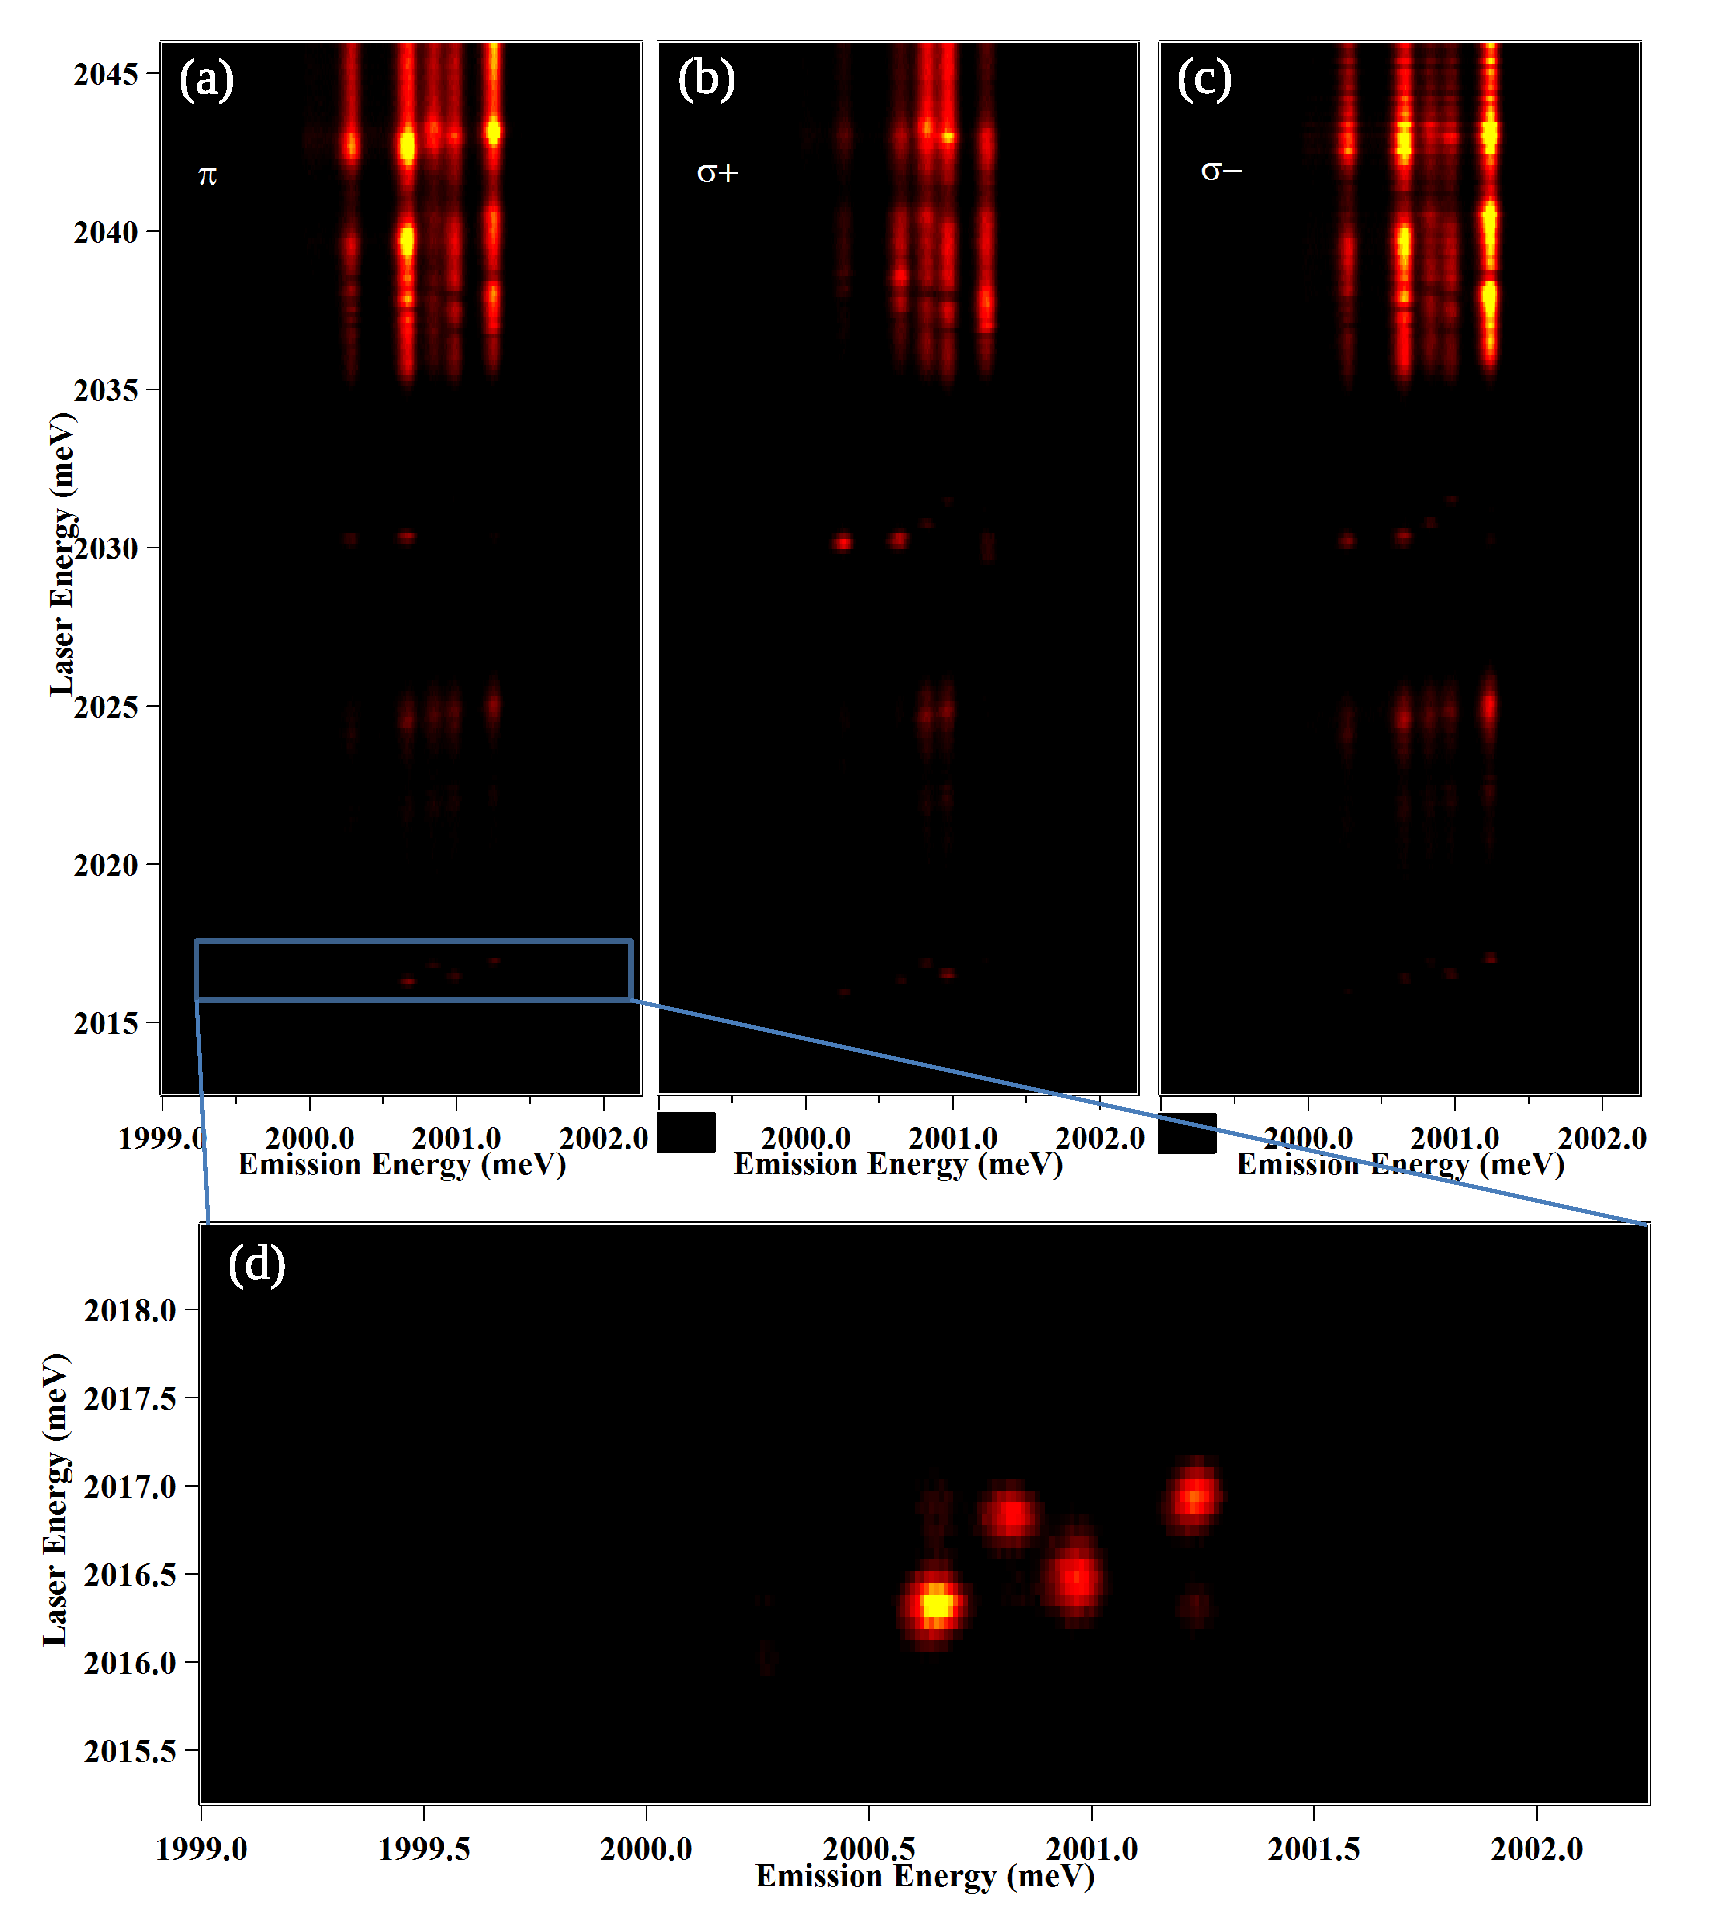
\includegraphics[width=12cm]{Pictures/PLE2030.eps}
%	\end{center}
%	\caption{(a) - (c) PLE map between 2046 meV and 2013 meV presenting several excited, detecting in $\pi$ (a),  $\sigma_{co}$ (b) and $\sigma_{cross}$ (c). (d) Zoom in a particular excited state presented a splitting inversion, taken in $\pi$ detection.}
%	\label{PLE2030}
%	\end{figure}
	
	At higher excitation energy, several excited states appear. The lower energy one is around 2018.5 meV, zoomed in on Fig.~\ref{FullPLE}(e). On this excited state, each peak presents a slightly different resonant energy. One can see that the order of appearance of the two central peaks seems to be reversed compared to the external ones. This phenomenon was first observed on QDs in GaAs quantum well~\cite{FineStructSplitGaAsdots}. This indicates an inversion of the splitting and is likely due to the electron-hole exchange interaction~\cite{SplitInvTh}.
	
	Another excited state can be saw at 2025 meV. This excited state occurs on a large energy band and can be linked back to an excitation to the optical phonon. Looking at the $\sigma$ polarized emission of this state (Fig.~\ref{PLEDotPres}(b) and (c)), we can see that the low and high energy peaks are strongly $\sigma$ polarized, while the central peaks do not show dependency over circular polarization. This, once again, show the good spin conservation of the system, as highlighted on the quasi-resonant state. 
	
	Finally, another interesting excited state appear at 2030 meV. This state presents an exchange-induced splitting  different from the splitting in the quasi-resonant state. This is due to a difference in the carriers and Cr atom wavefunction overlap. One can also noticed the this state presents a stronger luminescence in $\sigma_{cross}$ than in $\sigma_{co}$, [TO REDISCUSS] hinting at a spin flip of the hole before the recombination.
		
		\subsection{Magneto-optics of a quantum dot doped with a single Cr\label{MagOptCr}}
		
	The structure of the energy levels in Cr-doped QDs is confirmed by the evolution of the PL spectra in magnetic field (up to 11T) along the growth axis, the so called in Faraday configuration~\cite{BesombesPumpMnSFD}, presented in Fig.~\ref{CrMagOptExp}. Under magnetic field, the bright exciton $X_z = \pm1$ split, leading to a $\sigma-$ brach going at low energy and a $\sigma+$ one going at high energy. This splitting of the exciton of the exciton under magnetic field can compensate the one induced by the exchange interaction with the Cr~\cite{LegerQDGeomEffect}. For QD1, this results in an anti-crossing of $|+1\rangle$ and $|-1\rangle$ excitons due to the e-h exchange interaction around B$_z$=6 T observed both in $\sigma+$ and $\sigma-$ polarizations (anti-crossing (2) and (3) in Fig.~\ref{CrMagOptExp}(a)).
		
	\begin{figure}[h!]
	\begin{center}
		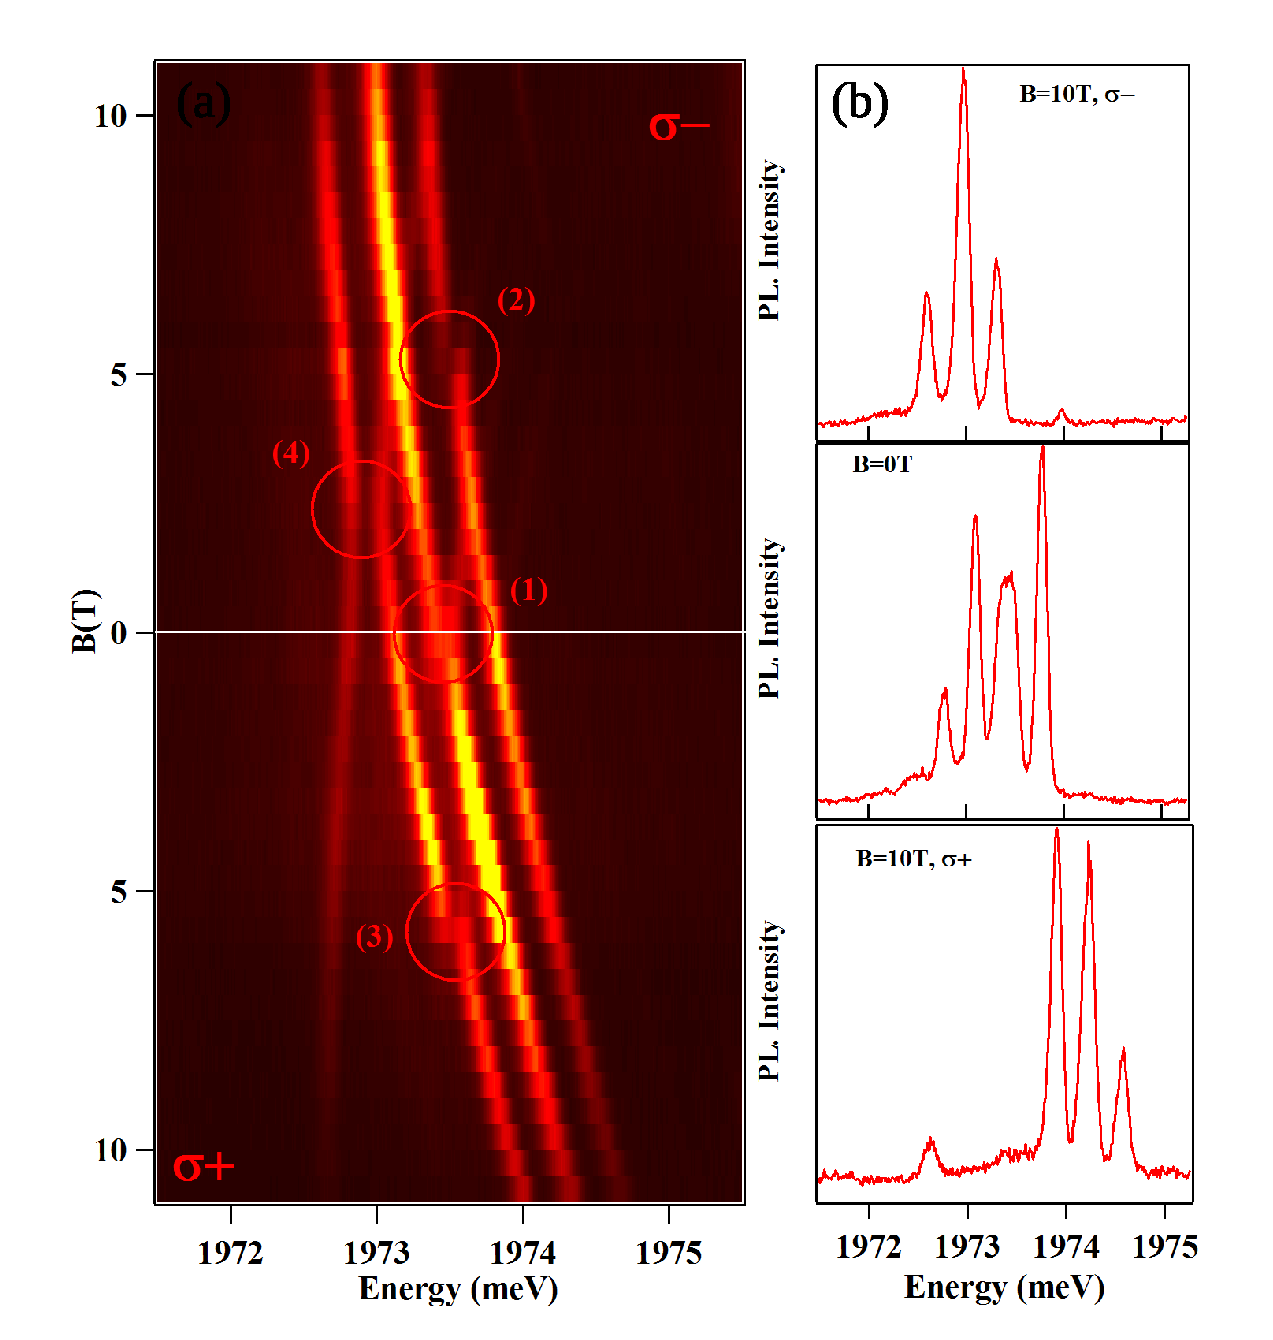
\includegraphics[width=10cm]{Pictures/MagOptv2.eps}
	\end{center}
	\caption{(a) Circularly polarized X-Cr PL evolution under magnetic field ($B_z$) in QD1. Anti-crossings  are highlighted and numbered. (b) QD1 X-Cr PL spectra taken at 0 and $10$T for both circular polarization.}
	\label{CrMagOptExp}
	\end{figure}
		
		The low energy emission presented as a dark exciton in Fig.~\ref{CrDecay} shows an anti-crossing with the bright excitons under $B_z$ in $\sigma-$ polarization (anti-crossing (4) in Fig.~\ref{CrMagOptExp}). As illustrated in Fig.~\ref{CrMagOptMod}(b), this anti-crossing arises from a mixing of the bright and dark excitons interacting with the same Cr spin state. Observed in $\sigma-$ polarization, it corresponds to the mixing of the exciton states $|-1\rangle$ and $|+2\rangle$ coupled to the Cr spin $S_z=-1$. This dark/bright excitons coupling $\delta_{12}$ is induced by the e-h exchange interaction in a confining potential of reduced symmetry (lower than C$_{2v}$)~\cite{DERecombTh}. In such symmetry, the dark exciton acquire an in-plane dipole moment which leads to possible optical recombination at zero magnetic field~\cite{DELum} as observed in these QDs. The oscillator strength of this "dark exciton" increases as the initial splitting between $|-1\rangle$ and $|+2\rangle$ excitons is reduced by the magnetic field (Fig.~\ref{CrMagOptMod}(b)).
		
	\begin{figure}[h!]
	\begin{center}
		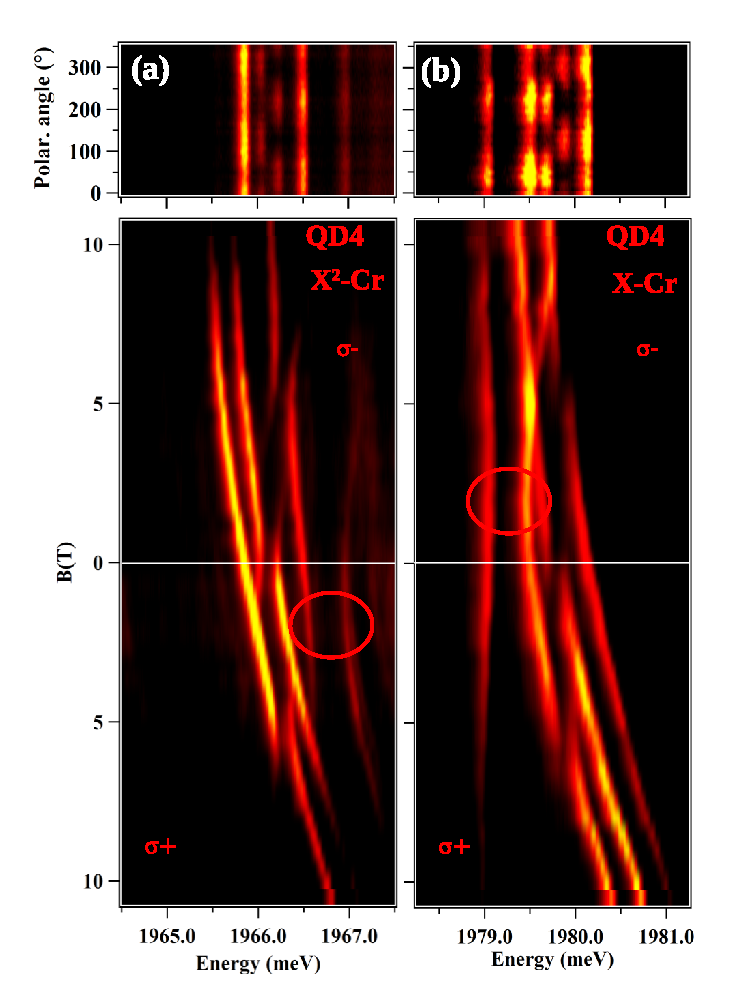
\includegraphics[width=10cm]{Pictures/MagOptLowSym.eps}
	\end{center}
	\caption{Linear polarization intensity map (top panel) and intensity map of the longitudinal magnetic field dependence of the emission (bottom panel) of (a) X$^2$-Cr and (b) X-Cr in QD3.}
	\label{CrMagOptLowSym}
	\end{figure}
		
		To illustrate the influence of the QD symmetry on the magneto-optical properties of X-Cr, we show in Fig.~\ref{CrMagOptLowSym}(b) the emission of a QD with a different strain state (QD3). For QD1, the splitting of the central peak is not clear in the PL at 0T (Fig.~\ref{SpectraX}(a)) without the linear polarization map, while two linearly polarized peaks appears clearly in QD3 spectra. This difference in emission arise from a difference in the in-plane strain of each QD~\cite{SplitInvTh}. The dark exciton emission is also stronger in QD2, confirming a lower symmetry than QD1.
		
		Investigating both the biexciton and the exciton in the same Cr-doped QD, we can also analyze the impact of the carrier-Cr interaction on the fine structure of the Cr spin. The magnetic field dependency of X$^2$-Cr emission in QD3 is presented along with the X-Cr emission as a contour plot in Fig.~\ref{CrMagOptLowSym}(a) and (b) respectively. The PL under magnetic field of X-Cr and X$^2$-Cr present a mirror symmetry. In particular, the dark/bright exciton mixing observed around $B_z$=2.5T on the low energy side of the PL in $\sigma-$ polarization for X-Cr is observed on the high energy side in $\sigma+$ polarization for X$^2$-Cr (circles in Fig.~\ref{CrMagOptLowSym}(a) and (b)).
		
	\begin{figure}[h!]
	\begin{center}
		\includegraphics[width=10cm]{Pictures/Antiferro-Cr.eps}
	\end{center}
	\caption{(a) Evolution in magnetic field of QD4 X-Cr circularly polarized PL. (b) Highlight of the PL evolution at $B_z = 0$T and $B_z = 7$T in both polarization. }
	\label{CrAntiferro}
	\end{figure}
		
		If one consider the ground state of X$^2$ as a spin-singlet (total spin 0), it cannot be split by the magnetic field or the spin interaction part of the carriers-Cr hamiltonian. The creation of two excitons in the QD cancels the exchange interaction with the Cr atom. Thus, the PL of  X$^2$-Cr is controlled by the final state of the optical transitions, i.e. the eigenstates of X-Cr, resulting in the observed mirror symmetry in the PL spectra. However, in some of the QDs, the X$^2$-Cr emission slightly deviates from this simple picture: a smaller energy splitting is observed for X$^2$-Cr compared to X-Cr (see X-Cr and X$^2$-Cr in Fig.~\ref{CrMagOptLowSym}). This shows that there is an interaction of X$^2$ with the Cr atom. It could result from a perturbation of the carriers' wave function by the interaction with the magnetic atom~\cite{CarInSpinSplit,BiexFinStruct} or a modification the local electric field which controls the Cr fine structure. [TO BE INVESTIGATED]
		
	\begin{figure}[h!]
	\begin{center}
		\includegraphics[width=10cm]{Pictures/Antiferro-Mn.eps}
	\end{center}
	\caption{(a) Evolution in magnetic field of the PL of a single Manganese atom coupled to an exciton in a II-VI QD. (b) PL spectra of the X-Mn system taken at $B_z = 0$T and $B_z = 11$T in both circular polarization. These experimental results are taken from Yoan L\'eger PhD thesis~\cite{YoanTh}.}
	\label{MnAntiferro}
	\end{figure}
		
	The evolution under magnetic field of the relative intensity of each of the QD peak gives information on the sign of the interaction between the Cr and the hole. As shown in Fig.~\ref{CrEnergyStruct}, given a polarization, each peak can be linked to a Cr spin state. As discussed earlier, applying a magnetic field lift the degeneracy between the exciton states and allow to efficiently select the polarization of the emission. For QD1, as shown in Fig.~\ref{CrMagOptExp}, all peaks keep the same emission intensity throughout the entire map. It hints for a high spin effective temperature, mediated by out of equilibrium phonons, allowing for high energy states to be populated.
	
	QD3, (Fig.~\ref{CrMagOptLowSym}) and QD4 (Fig.~\ref{CrAntiferro}) presents a better thermalisation and thus shows a clearer evolution of the intensity under magnetic field. The $S_z = 0$ state is not affected by the magnetic field and stays the lower spins state for the Cr atom. Therefore, it stays populated for all values and orientations of the magnetic field. The picture is different for the exterior peaks. In the $\sigma-$ branch, the high energy peak get brighter while the low energy one disappear for $B_z \geq 8$T in QD4. The situation is opposite in the $\sigma+$ branch, where the intensity concentrate on the lower energy peak. This evolution is the same at the one found for single Mn atoms in II-VI QDs~\ref{MnAntiferro}. It was shown in Yoan L\'eger PhD thesis~\cite{YoanTh} that the $S_z = -\frac{5}{2}$ state of the Mn atom was stabilized under magnetic field. From this evolution and the polarization of the different Mn states, it was then possible to deduce the interaction between Mn and hole was anti-ferromagnetic.
	
	The situation of Cr is similar. Under magnetic field, the $S_z = -1$ is stabilized, becoming the lower energy state of the doublet $S_z = \pm1$. For a magnetic field high enough for the other peak to disappear ($B_z = 8$T in QD4), we can consider the states linked to $S_z = +1$ to be emptied and only consider the $S_z = +1$ ones. The high energy transition corresponds then to the $|S_z = -1, X_z = -1\rangle \rightarrow |S_z = -1\rangle$ on, in $\sigma-$ polarization, while the low energy peak is associate with the $|S_z = -1, X_z = +1\rangle \rightarrow |S_z = -1\rangle$ transition, in $\sigma+$ polarization. This is coherent with an anti-ferromagnetic coupling between the Cr and hole, and confirm the energy structure presented in Fig.~\ref{CrEnergyStruct}.
		
	\section{Modelization of a Cr-doped QD\label{QDParam}}
		
	\begin{figure}[h!]
	\begin{center}
		\includegraphics[width=15cm]{Pictures/SimuAntiferro.png}
	\end{center}
	\caption{(a) Up: Calculated linear polarization PL intensity map of X-Cr at zero field. The 0$^{\circ}$ polarization angle correspond to an emission polarized along the $100$ axis. Down: Calculated X-Cr circularly polarized magnetic field dependency. Details of the model and parameters are listed in Tab.~\ref{CrModelParam}. Corresponding anti-crossing are highlighted in same fashion as on Fig.~\ref{CrMagOptExp} and \ref{CrAntiferro}. On the right, spectra taken for $B_z = 0$T and $B_z = 11$T in both circular polarization are shown. (b) Schema of the magnetic field dependency of the energy levels of the low energy Cr spin states $S_z$=0 and $S_z$=$\pm$1, and corresponding bright ($|+1\rangle$ blue, $|-1\rangle$ red) and dark ($|\pm2\rangle$ green) X-Cr energy levels.}
	\label{CrMagOptMod}
	\end{figure}
	
	We calculated the magneto-optic behaviour of Cr-doped QDs by diagonalizing the complete Hamiltonian of the e-h-Cr in self-assembled dots. This hamiltonian can be separated as follows:
	
	\begin{align}
\label{X-Cr} {\cal H}_{X-Cr}={\cal H}_{Cr,\varepsilon}+{\cal H}_{cCr}+{\cal H}_{mag}+{\cal H}_{eh}+{\cal H}_{band}+{\cal H}_{scat}
	\end{align}
where:

${\cal H}_{Cr,\varepsilon}$ describes the fine structure of the Cr atom and its dependency on local strain, as presented in Eq.~\ref{Cralone}. It is mainly drived by $D_0$, the magnetic anisotropy. E, the in-plane strains, also appears in this Hamiltonian, but have to be kept small in order to model the found dots (see Fig.~\ref{CrHighE} for the emission of a dot with a higher E).

${\cal H}_{cCr}$ describes the coupling of the electron and hole with the Cr spin, depending on $I_{eCr}$, the exchange integral of the electron-Cr spins, and $I_{hCr}$, the exchange integral of the hole-Cr spins, as described in Eq.~\ref{HCrDMS}.

${\cal H}_{mag}$ describes the effect of an exterior magnetic field, coupled to both the Cr and carrier spins by the Zeeman terms, depending on the $g$-factor of each of them and the Bohr magneton $\mu_B$, and including the diamagnetic shift of the electron-hole via the term $\gamma$.
\begin{align}
	{\cal H}_{mag} = g_{Cr}\mu_B\overrightarrow{B}.\overrightarrow{S}+g_{e}\mu_B\overrightarrow{B}.\overrightarrow{\sigma}+g_{h}\mu_B\overrightarrow{B}.\overrightarrow{J}+\gamma B^2
\end{align}

${\cal H}_{eh}$ describes the short range and long range electron-hole interaction, through the bright and dark exciton splitting $\delta_0$, the bright exciton coupling $\delta_1$, the dark exciton coupling $\delta_2$ and the bright and dark exciton coupling $\delta_{11}$ and $\delta_{12}$. All of these term are described in Eq~\ref{Heh}.

${\cal H}_{band}$ is the band Hamiltonian. It is written ${\cal H}_{band} = E_g + {\cal H}_{VBM}$, with $E_g$ the CdTe gap energy and ${\cal H}_{VBM}$ is described in Eq.~\ref{HVBM}.

${\cal H}_{scat}$ describes the perturbation of the wave function of the exciton in the initial state of the optical transition by the hole-Cr exchange interaction, controlled by the parameter $\eta$. This perturbation depends on the value of the exchange energy between the Cr spin $S_z$  and the hole spin $J_z$ and can be represented, using second order perturbation theory, by an effective spin Hamiltonian \cite{CarInSpinSplit,BiexFinStruct,DynhMn}
\begin{align}
{\cal H}_{scat}=-\eta S_z^2
\end{align}
\noindent with $\eta>0$.

	We considered the general case of QDs with a symmetry lower than C$_{2v}$ (truncated ellipsoidal lens for instance~\cite{DERecombTh}), and took into account the influence of this reduced symmetry on the valence band and on the e-h exchange interaction. The population of the X-Cr spin states split by the large magnetic anisotropy and the carriers-Cr exchange interaction is described by a spin effective temperature T$_{eff}$. The results of the model obtained with T$_{eff}$=20K, $D_0$=2.2 meV and an electron-Cr (hole-Cr) exchange interaction $I_{eCr}$=-50$\mu$eV ($I_{hCr}$=250 $\mu$eV) are reported in Fig.~\ref{CrMagOptMod} (parameters not specific to Cr-doped QDs are listed in Tab.~\ref{CrModelParam}). Such parameters do not aim to fit the data and are only reasonable order of magnitude. The PL of X-Cr at zero field and its evolution in magnetic field can be qualitatively reproduced. In particular, the description of the spin states occupation by T$_{eff}$ is sufficient to reproduce the observed emission from the three low energy X-Cr levels (Cr spin states $S_z = |0\rangle$ and $S_z = |\pm1\rangle$). The splitting of the central line at zero field (anti-crossing (1)) and the anti-crossings under magnetic field (anti-crossings (2) and (3) around $B_z$=6T for the Cr spin states  $S_z = |+1\rangle$ and anti-crossings (4) with the dark exciton around $B_z$=2T) are also well reproduced by the model. 
	
	This simulation predicts an anti-crossing around $B_z = 5$T, noted (5) and caused by an electron-Cr flip flop, which is not sawn on the experiment. Its position is controlled by $D_0$ and its intensity by $I_{eCr}$. However, for this anti-crossing to appear for $B_z > 11$T, a $D_0 > 3$ meV is needed, causing the $S_z = |\pm1\rangle$ levels to be at high energy and thus giving a stronger emission intensity to the $S_z = 0$ state than the one saw in the experiments. Therefore, a low value of $I_{eCr}$ was chosen instead. Finally, the remaining tail of an anti-crossing, labelled (6), also appears at high magnetic field in the $\sigma-$ polarization, as saw in Fig.~\ref{CrAntiferro}, due to the coupling a bright and a dark exciton coupled to the Cr state $S_z = |0\rangle$.

	
%	\begin{table}[t] \centering
%	\caption{Values of the parameters used in the model of Cr-doped CdTe/ZnTe quantum dot presented in Fig.~\ref{SpectraX}(b). The value of the parameters not listed in the table is 0. The chosen values are typical for CdTe/ZnTe quantum dots and can be compared with parameters extracted from Mn-doped quantum dots \cite{DynhMn,DELum}. These values are reasonable to reproduce the emission of the QDs presented in this thesis.}
%	\renewcommand{\arraystretch}{1.0}
%	\begin{tabular}{p{0.9cm}p{0.9cm}p{0.9cm}p{0.9cm}p{0.9cm}p{0.9cm}p{0.9cm}p{0.9cm}p{0.9cm}p{0.9cm}p{0.9cm}p{0.9cm}p{0.9cm}p{1.3cm}
%p{0.9cm}p{0.9cm}}
%\hline\hline
%I$_{eCr}$ & I$_{hCr}$ & $\delta_0$ & $\delta_1$ & $\delta_{12}$ & $\delta_{11}$ & $\frac{|Q|}{\Delta_{lh}}$ & $\frac{|R|}{\Delta_{lh}}$ & arg(R) & $D_0$ & $g_{Cr}$ & $g_{e}$ & $g_{h}$ & $\gamma$ & $\eta$ & $T_{eff}$ \\
%$\mu eV$ & $\mu eV$ & $meV$ & $\mu eV$ & $\mu eV$ & $\mu eV$ &  & & & $meV$ & &  &  & $\mu eV/T^2$ & $\mu eV$ & K \\
%\hline
%-70 & -280 & -1 & 250 & 150 & 50 & 0.05 & 0.05& $-\frac{\pi}{2}$ & 2.5 & 2 & -0.7 & 0.4 & 1.5 & 25 & 25 \\
%\hline\hline 
%	\end{tabular}
%	\label{CrModelParam}
%	\end{table}

%\begin{wraptable}{r}{5.5cm}
%	\caption{Values of the parameters used in the model of Cr-doped CdTe/ZnTe quantum dot presented in Fig.~\ref{SpectraX}(b). The value of the parameters not listed in the table is 0. The chosen values are typical for CdTe/ZnTe quantum dots and can be compared with parameters extracted from Mn-doped quantum dots \cite{DynhMn,DELum}. These values are reasonable to reproduce the emission of the QDs presented in this thesis.}
%	\renewcommand{\arraystretch}{1.0}
%	\begin{tabular}{m{1.3cm}|m{1.3cm}||m{1.3cm}}
%I$_{eCr}$ & $\mu eV$ & -70\newline \\
%I$_{hCr}$ & $\mu eV$ & -280\newline \\
%$\delta_0$ & $meV$ & -1\newline \\
%$\delta_1$ & $\mu eV$ & 250\newline \\
%$\delta_{12}$ & $\mu eV$ & 150\newline \\
%$\delta_{11}$ & $\mu eV$ & 50\newline \\
%$\frac{|Q|}{\Delta_{lh}}$ &  & 0.05\newline \\
%$\frac{|R|}{\Delta_{lh}}$ &  & 0.05\newline \\
%arg(R) &  & $-\frac{\pi}{2}$\newline \\
%$D_0$ & $meV$ & 2.5\newline \\
%$g_{Cr}$ &  & 2\newline \\
%$g_{e}$ &  & -0.7\newline \\
%$g_{h}$ &  & 0.4\newline \\
%$\gamma$ & $\mu eV/T^2$ & 1.5\newline \\
%$\eta$ & $\mu eV$ & 25\newline \\
%$T_{eff}$ & K & 25\newline \\
%	\end{tabular}
%	\label{CrModelParam}
%	\end{wraptable}

\begin{table}[t] \centering
	\caption{Values of the parameters used in the model of Cr-doped CdTe/ZnTe quantum dot presented in Fig.~\ref{CrMagOptMod}. The value of the parameters not listed in the table is 0. The chosen values are typical for CdTe/ZnTe quantum dots and can be compared with parameters extracted from Mn-doped quantum dots \cite{DynhMn,DELum}. These values are reasonable to reproduce the emission of the QDs presented in this thesis.}
	\renewcommand{\arraystretch}{1.0}
	\begin{tabular}{p{0.9cm}p{0.9cm}p{0.9cm}p{0.9cm}p{0.9cm}p{0.9cm}p{0.9cm}p{0.9cm}}
\hline\hline
I$_{eCr}$ & I$_{hCr}$ & $\delta_0$ & $\delta_1$ & $\delta_{12}$ & $\delta_{11}$ & $\frac{|Q|}{\Delta_{lh}}$ & $\frac{|R|}{\Delta_{lh}}$ \\
$\mu eV$ & $\mu eV$ & $meV$ & $\mu eV$ & $\mu eV$ & $\mu eV$ &  & \\
\hline
-50 & -250 & -1 & 250 & 150 & 50 & 0.05 & 0.05 \\
\hline\hline 
	\end{tabular}
	\begin{tabular}{p{0.9cm}p{0.9cm}p{0.9cm}p{0.9cm}p{0.9cm}p{1.3cm}p{0.9cm}p{0.9cm}}
arg(R) & $D_0$ & $g_{Cr}$ & $g_{e}$ & $g_{h}$ & $\gamma$ & $\eta$ & $T_{eff}$ \\
 & $meV$ & &  &  & $\mu eV/T^2$ & $\mu eV$ & K \\
\hline
$-\frac{\pi}{2}$ & 2.2 & 2 & -1 & 0.4 & 1.5 & 25 & 20 \\
\hline\hline
	\end{tabular}
	\label{CrModelParam}
	\end{table}
	
	The magnetic anisotropy $D_0$ cannot be precisely extracted from the PL spectra. However, for $D_0 <  2$ meV, an anti-crossing due to a VBM induced hole-Cr flip-flop between the $|-1, +2\rangle$ and the $|0, -1\rangle$ would appear below B$_z$=11T on the central line in $\sigma-$ polarization. Moreover, as discussed earlier, a higher value of $D_0$ would produce a lower PL intensity for the states $S_z = |\pm1\rangle$. These consideration sets a $D_0$ in the range of 2 to 3 meV. However, even in this range, the intensity distribution of the PL cannot be perfectly reproduced: while the intensity ratio of the peaks is quite well predicted for high value of the magnetic field, the $S_z = |0\rangle$ state still present a stronger emission at $B_z = 0$T than the one observed in the experiment. This difference in intensity may be due to out of equilibrium phonons in the sample that help populating the $S_z = |\pm1\rangle$ states.

	Our model reproduce qualitatively with enough satisfaction the data found experimentally and thus can be used to see the evolution of the emission varying different parameter. Especially, an interesting point is the influence of the anisotropy of strains on the emission. This simulation was done by applying a small magnetic anisotropy $D_x$ along the $x$ axis of the quantum dot and none along the $y$ axis ($D_y$=0), equating to an effective $E$. Results of such a study are presented on Fig.~\ref{CrHighE}, (a) and (b) for the X-Cr system, and (c) and (d) for the X$^c$-Cr one.
	
	\begin{figure}[h!]
	\begin{center}
		\includegraphics[width=10cm]{Pictures/HighE.eps}
	\end{center}
	\caption{For a QD with a small magnetic anisotropy along the $x$ axis (D$_x$ = 150 $\mu$eV, D$_y$ = 0 $\mu$eV,  D$_z$ = 2500 $\mu$eV): (a) (resp. (c)) calculated X-Cr (resp. X$^c$-Cr) linear polarization PL intensity at 0T; (b) (resp. (d)) calculated X-Cr (resp. X$^c$-Cr) circularly polarized magnetic field dependency.}
	\label{CrHighE}
	\end{figure}
	
	The X-Cr map in linear polarization shows a splitting of all the three peaks at 0T, when only the central  peaks exhibit this behaviour in dots with a small in-plane anisotropy at the Cr position. The effect of such an anisotropy is to coupled to spin levels separated by two spin units, such as $|S_z = -1\rangle$ and $|S_z = +1\rangle$. This induce a mixing between two bright exciton states, leading to a linearly polarized emission. For a low $E$ value, the strain induced splitting of $|S_z = \pm 1\rangle$ is high enough to strongly reduce the mixing of the exciton states. A higher in-plane strain anisotropy is able to couple the spin level and induced the linearly polarized emission.

%	The first remarkable feature appear on the linear polarization dependency of the X-Cr system(Fig.~\ref{CrHighE}(a)). While, with a small value of E, only the $|0\rangle$ peaks presents linear polarization, at higher value, $|\pm 1\rangle$ peaks presents the same behaviour.
	
	X$^c$-Cr, as said in Sec.~\ref{ehExch}, is not affected by the e-h exchange interaction, and thus does not present any linear polarization dependency, as shown on Fig.~\ref{CrHighE}(c).
	
	The evolution of the emission under magnetic field also presents different characteristics than a QD with magnetic anisotropy purely along z. Fig.~\ref{CrHighE}(b) presents the evolution in B of the X-Cr emission. 
One can note anti-crossings at +5T appearing on both $|S_z = +1\rangle$ and $|S_z = -1\rangle$, as well as an anti-crossing at -5T appearing on the low energy emission lines. These are similar to the anti-crossing (2), (3) and (4) on Fig.~\ref{CrMagOptMod}. Around 0T, other anti-crossings appear, on all the three peaks this time. Anti-crossing on the central peaks is the same as the anti-crossing (1) in Fig.~\ref{CrMagOptMod}. The ones appearing on the $|S_z = \pm 1\rangle$ peaks arise from the exciton mixing via $E$, as evidenced by the linear polarization.

	X$^c$-Cr in dot with high in-plane anisotropy at the Cr position also presents anti-crossing for a magnetic field around 1T, as shown in Fig.~\ref{CrHighE}(d). This anti-crossing appears when the Zeeman effect of the Cr atom compensates the electron-Chromium interaction and the hole-Chromium interaction.
				
	
	\section{Charge fluctuation of a Cr ion  in the vicinity  of the QDs}
	
	Some dots were found presenting a linear polarization dependency both on their central peaks and on their exterior peaks. However, such dots didn't present any anti-crossing when probed under magnetic field. Results of these experiments are presented in Fig.~\ref{CrSixPeaksMagOpt}.
	
	\begin{figure}[h!]
	\begin{center}
		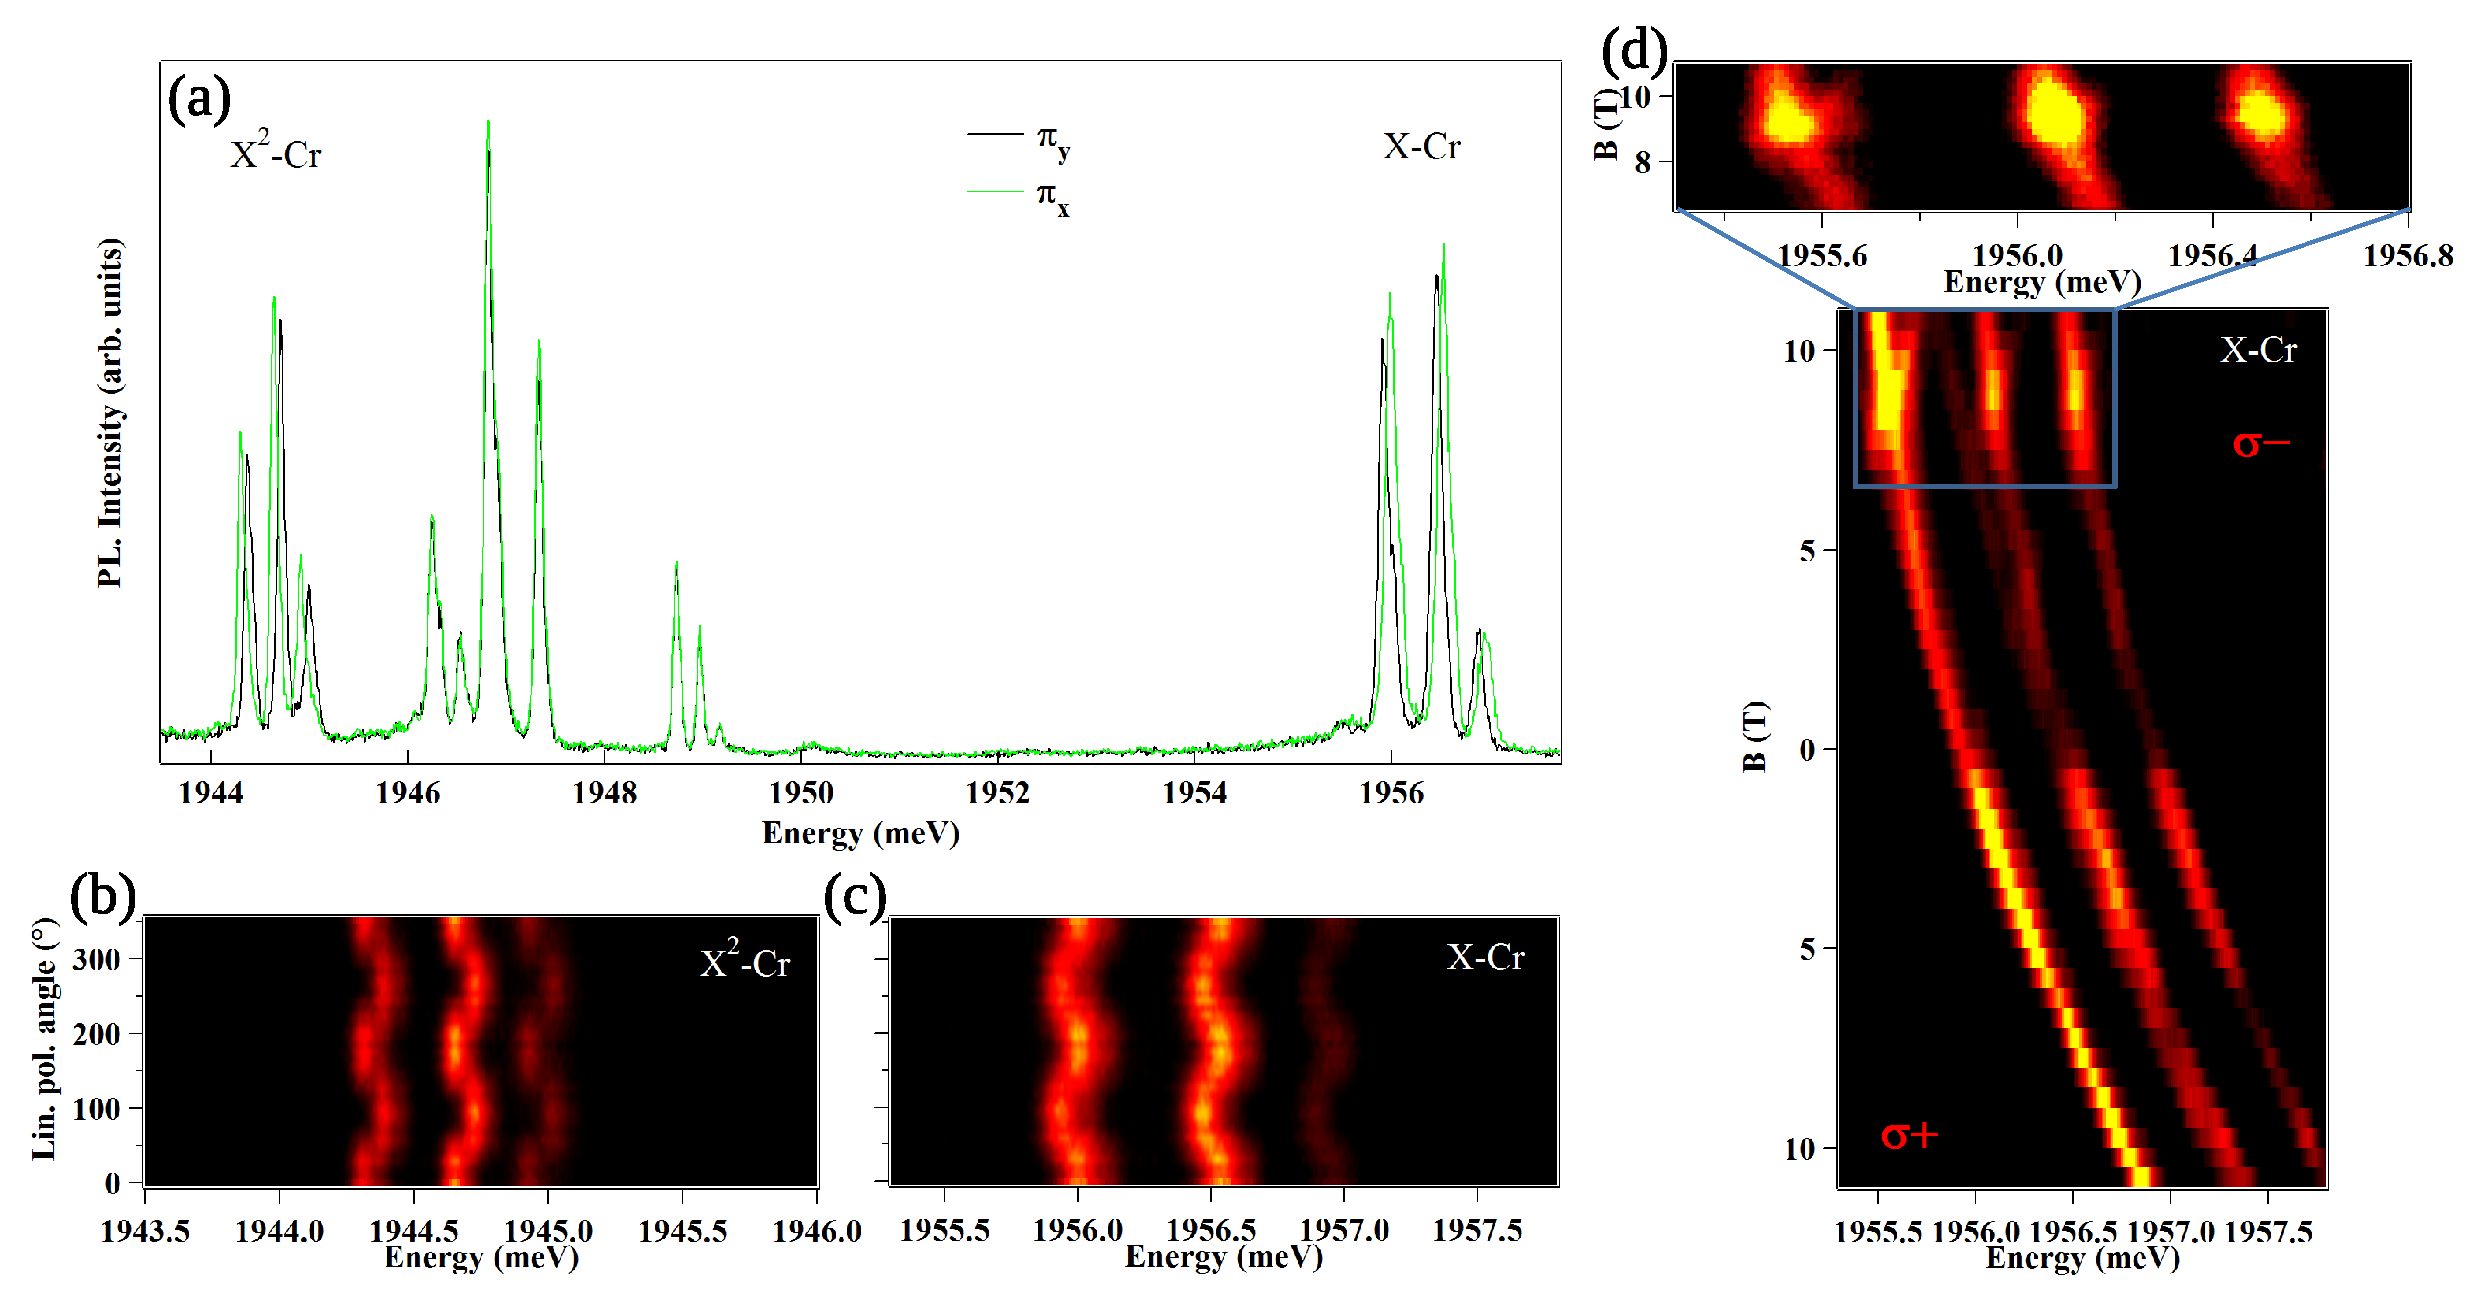
\includegraphics[width=15cm]{Pictures/6peaks.eps}
	\end{center}
	\caption{(a) QD5 linearly polarized PL intensity at zero magnetic field. (b) and (c) Respectively QD6 X$^2$-Cr and X-Cr linear polarization PL dependence at zero magnetic field. (c) X-Cr magnetic field PL dependence on this QD. Zoom in presents anti-crossing appearing at B=9T.}
	\label{CrSixPeaksMagOpt}
	\end{figure}
	
	A common feature of all of these dots is the thin and well split X$^+$-Cr PL structure, shown on Fig.~\ref{CrSixPeaksMagOpt}(a) around 1949mev. X-Cr and X$^2$-Cr also present three well defined peaks, with a broad emission. This is not a general case, as some dots were found presenting a broad emission on X-Cr and X$^2$-Cr positions, such as QD6 presented in Fig.~\ref{CrSixPeaksSplit}. The linear polarization map of the QD5 PL reveals that each peak presents a linear polarization dependency (Fig.~\ref{CrSixPeaksMagOpt}(b) and (c)).
	
	The PL evolution of such a dot is presented in Fig.~\ref{CrSixPeaksMagOpt}(d). The  diamagnetic shift is clearly visible. However, the only anti-crossings appear at B=9T for all the peaks (zoom in Fig.~\ref{CrSixPeaksMagOpt}(d)). Such anti-crossings are characteristic of an exciton in a QD with no magnetic atom: it arise from the dark and bright exciton mixing.
	
	\begin{figure}[h!]
	\begin{center}
		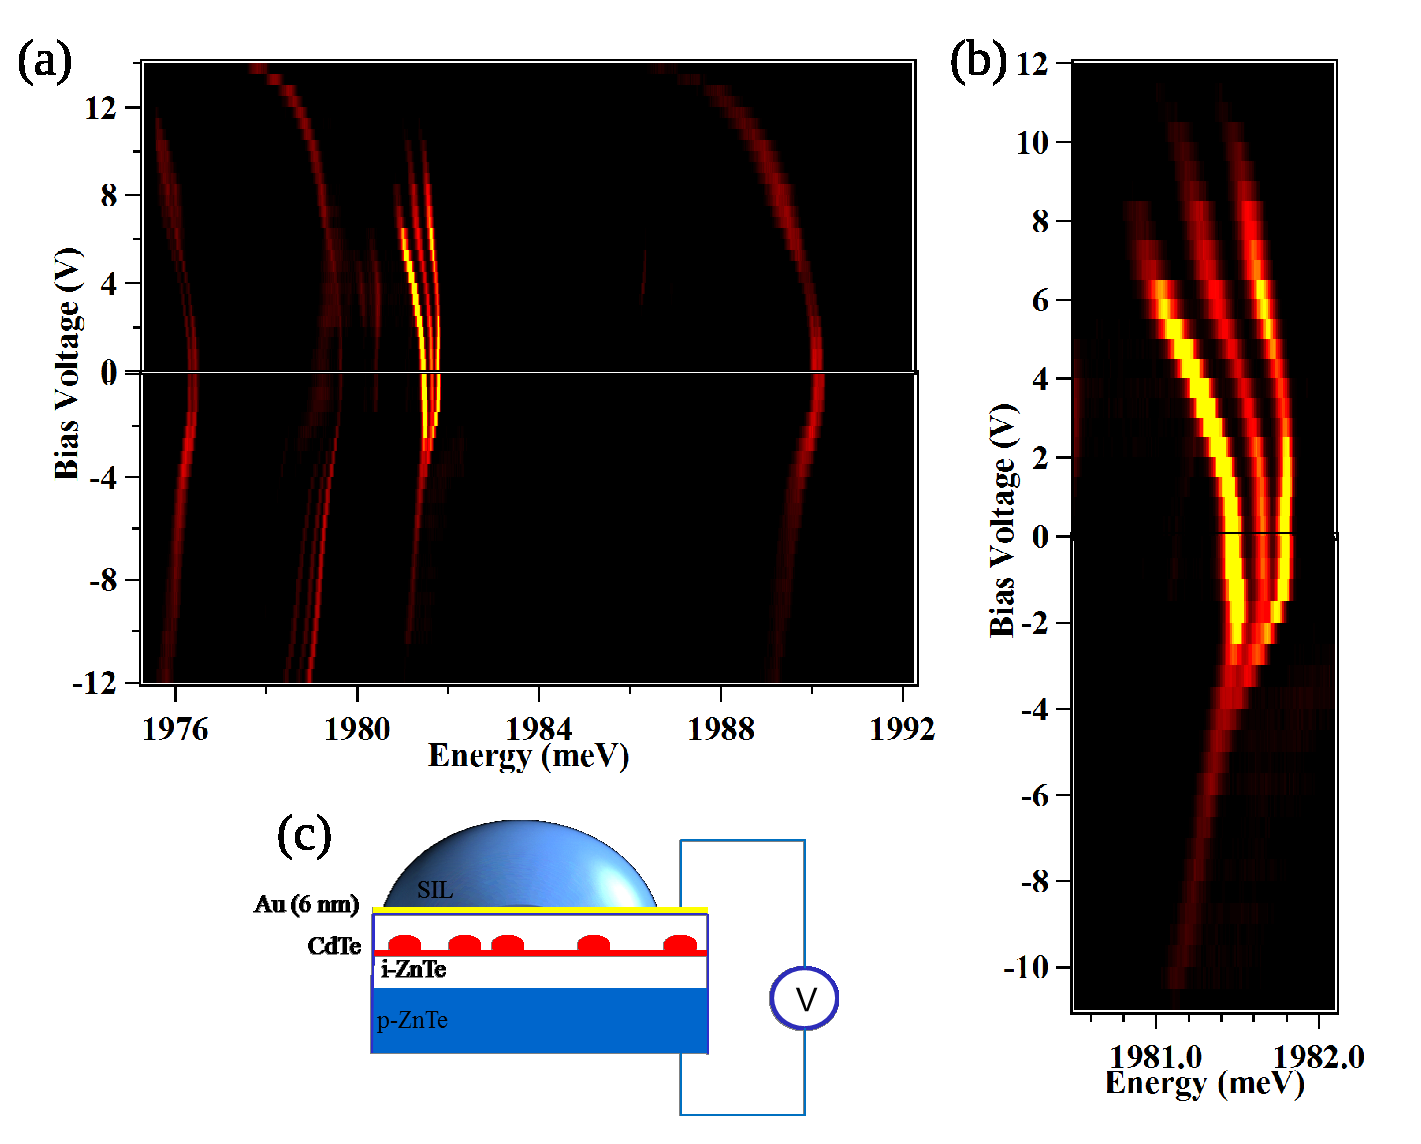
\includegraphics[width=12cm]{Pictures/EfieldX-Xc.eps}
	\end{center}
	\caption{(a) QD7 whole PL evolution under application of a bias voltage. (b) Zoom on X$^c$-Cr circular polarization PL intensity evolution under electric field. A strong stark shift is observed, as well as variation in the splitting. (c) Schema of a sample with a Schottky gate used to apply the bias voltage on the sample.}
	\label{CrSixPeaksEFieldX+}
	\end{figure}	
	
	In order to get more informations on these dots, it was decided to study them applying a bias voltage. The application of an electric field was realized via a sample with a Schottky gate in the same fashion than the one in Sec.~\ref{ChargeSelec}. The resulting map is presented in Fig.~\ref{CrSixPeaksEFieldX+}(a). The first visible feature is the strong electric field dependency of the emission energy, more marked for X-Cr than for the X$^c$-Cr systems. The emission energy variation of the X-Cr complex occurs on a 2.9 meV scale.
	
	There is another remarkable point on these maps, evidenced on the X$^+$-Cr complex on the Fig.~\ref{CrSixPeaksEFieldX+}(b): the splitting between each peak is changing with the applied electric field. The splitting between the high and low energy peaks varies from 0 meV for an applied bias voltage of -12V (no splitting) to 0.76 meV for 13V applied. This disappearance of the splitting for a certain bias voltage indicates that the overlap between the electron and the hole wave functions is changed by the application of an exterior electric field, to the point where they don't overlap at all.

	\begin{figure}[h!]
	\begin{center}
		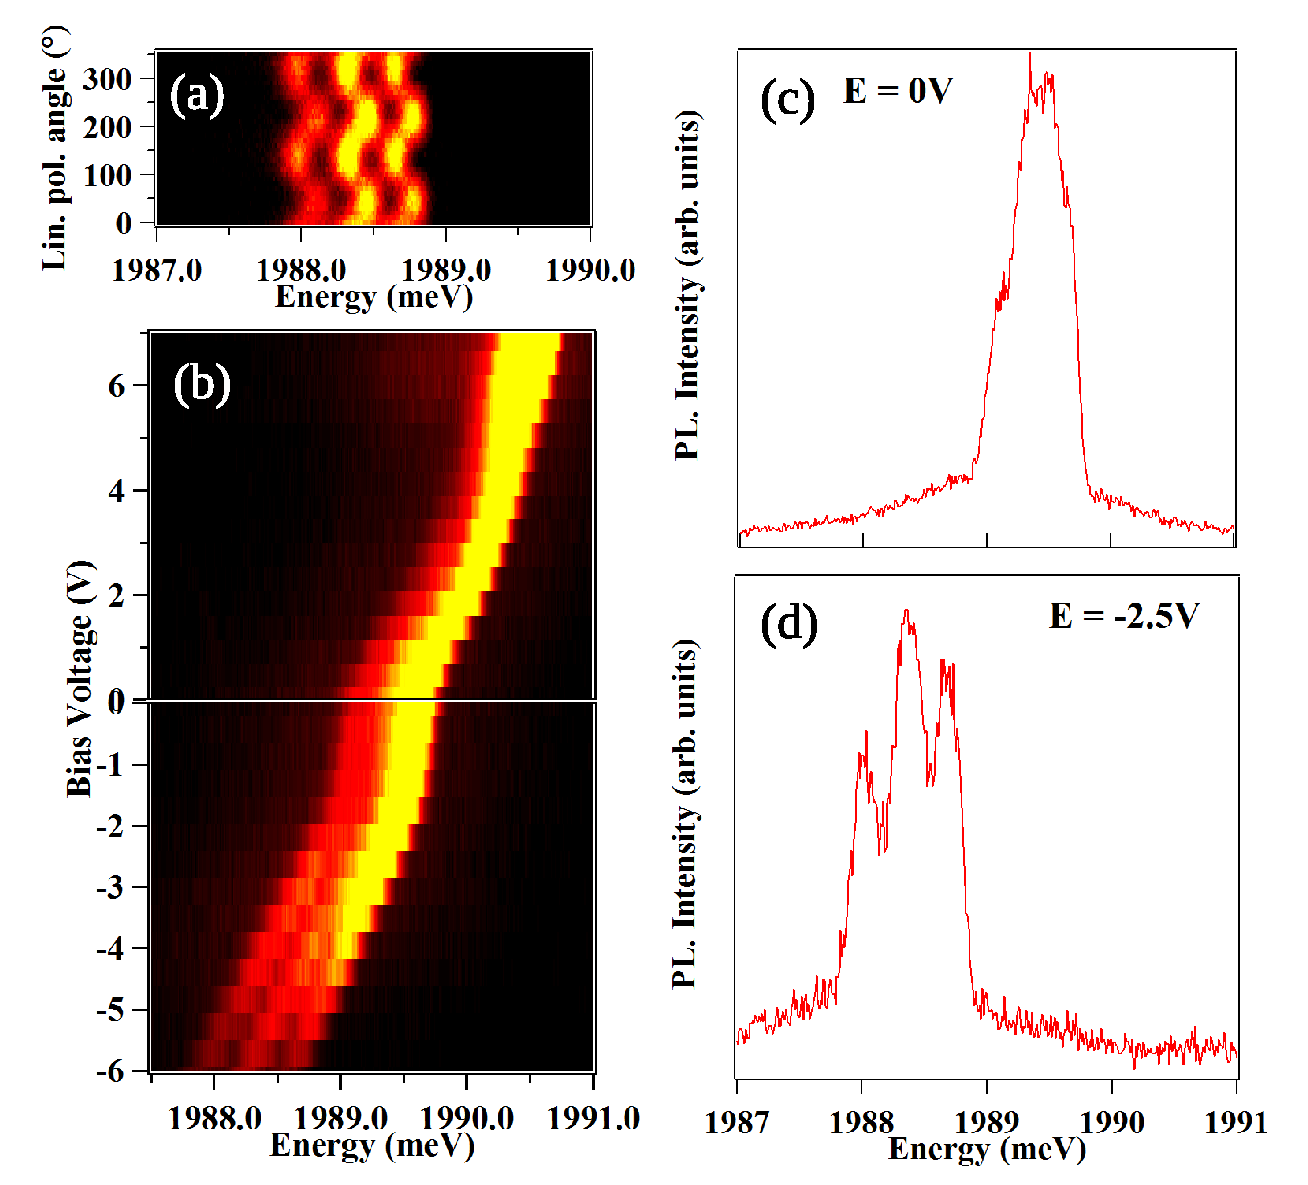
\includegraphics[width=12cm]{Pictures/SplitUnderEfiledXCr.eps}
	\end{center}
	\caption{All these measures were taken on QD8 X-Cr complex at low temperature. (a) PL intensity dependency in linear polarization. In order to have the best contrast, the map was taken at -2.5V bias voltage. (b) Circular PL intensity evolution in electric field. A splitting began to appear around -2V of applied bias voltage. (c)-(d) Circular PL for an applied bias voltage of, respectively, 0V and -2.5V.}
	\label{CrSixPeaksSplit}
	\end{figure}
		
	Fig.~\ref{CrSixPeaksSplit} shows that, using electric field, we can manipulate the splitting of any given charged state of the QD. For all positive bias voltage between 0V and 13V, X-Cr present a broad emission containing all six peaks in linear emission, as show on Fig.~\ref{CrSixPeaksSplit}(a). The emission then divide into three distinct peaks, starting to appear around -1V. This is evidenced on the the PL emission on Fig.~\ref{CrSixPeaksSplit}(d).
	
	\begin{figure}[h!]
	\begin{center}
		\includegraphics[width=15cm]{Pictures/CrCloseDot.png}
	\end{center}
	\caption{(a) Cr accessible charged states in ZnTe. (b)-(d) Illustration of the effect of a punctual charge on the wavefunction of an electron (red) and a hole (yellow) in a quantum dots.}
	\label{CrOutsideDot}
	\end{figure}
	
	This three peaks emission structure looks like a three levels system emitting at three different energies. However, the magnetic field evolution presented in Fig.~\ref{CrSixPeaksMagOpt}(c) does not reflect the presence of a magnetic atom in the quantum dot. Moreover, evolution under electric field shows huge changes in the carriers wave functions overlap. These features hint for a single exciton trapped in a QD presenting spectral fluctuations.
	
	Spectral fluctuations under a fluctuation of charge in the vicinity of a QD has been observed to lead to a peak broadening~\cite{ChargeSpectFluct}, such as observed on Fig.~\ref{CrSixPeaksSplit}(d), as well as spectrum jumps. For the PL to jump between three emission energies, the charge fluctuation has to be able to take three distinct charge values.
	
	Cr in ZnTe is incorporated as Cr$^{2+}$, but, as shown on Fig.\ref{CrOutsideDot}(a), the Cr$^+$ and Cr$^{3+}$ states are also accessible~\cite{CrZnTe}, either by capturing an electron (Cr$^+$) or a hole (Cr$^{3+}$). Considering such a charge close to the QD, it can be viewed as a punctual one, since the dot is far bigger than the atom. The effect on the wave functions, presented in Fig.\ref{CrOutsideDot}(b)-(d), differs depending on the electrical charge of the Cr atom. The electron is well confined in CdTe/ZnTe quantum dots, while the hole is almost not confined. Because of this, the electron wave function is almost not moved by the presence of the electric, when the hole one vary more depending on the charge state of the Cr. These differences in the overlapping of wave functions lead to three different emission energies depending on the Cr charge state.
	
	The charge variation of the Cr is of the value of the elementary charge. Considering a pure coulomb interaction between two punctual charges, for a charge at 5nm of the dot, its effect is of the same order of magnitude than the hole-Cr exchange interaction. In order to have a significant effect on the dot PL, the Cr has then to be close to it, not more than a few nanometres away. 
	
	This hypothesis is currently tested, along with the capacity for the Cr to diffuse outside the quantum dots layer.
	
	\section{Conclusion}
	
	For the first time, a single Cr atom in a semiconductor was probed optically. The fine structure of the Cr is dominated by a magnetic anisotropy induced by strain in the plane of the QDs. The large spin to strain coupling of Cr, two orders of magnitude larger than for magnetic elements without orbital momentum (NV centers in diamond \cite{SpinMechaDriv}, Mn atoms in II-VI semiconductors \cite{LafuenteStrainMn}) suggests some possible development of coherent mechanical spin-driving of an individual magnetic atom in a nano-mechanical oscillator. This new single spin system should allow, at low temperature, to enter some coupling regimes dominated by quantum coherent dynamics not reached until now in hybrid spin-mechanical devices.
	
	Some dots presents the same structure at 0T than dots containing a single Cr atom, but without presenting the signature of the presence of a magnetic atom under magnetic field. These dots are effected by the variation of charge of a single Cr atom in the barrier, close to the dot. Further study of the diffusion process of Cr in CdTe and ZnTe is required in order to avoid the creation of such dots.

\printbibliography

\end{document}
